% Copyright 2005-2016 Airbus-EDF-IMACS-Phimeca
% Permission is granted to copy, distribute and/or modify this document
% under the terms of the GNU Free Documentation License, Version 1.2
% or any later version published by the Free Software Foundation;
% with no Invariant Sections, no Front-Cover Texts, and no Back-Cover
% Texts.  A copy of the license is included in the section entitled "GNU
% Free Documentation License".

\documentclass[11pt]{article}

\usepackage{latex2html}
\usepackage{makeidx}
\usepackage{index}
\usepackage[dvips]{graphicx}
\usepackage{color}
\usepackage{longtable}
\usepackage{mdwtab}
\usepackage{hhline}
\usepackage{amsmath}
\usepackage{amssymb}
\usepackage{fancyhdr}

\usepackage{Math_Notations}
\usepackage{otcommon}

\newcommand{\requirements}[2]{{
    \noindent%
    \begin{tabular}{||p{2.3cm}||p{12.7cm}||}
      \hhline{|t:=:t:=:t|}
      Requirements\vfill & \parbox{12cm}{
        {\#1}
      } \\
      \hhline{|:=::=:|}
      Results\vfill      & \parbox{12cm}{
        {\#2}
      } \\
      \hhline{|b:=:b:=:b|}
    \end{tabular}
}}

\newcommand{\longrequirements}[2]{{
    \noindent%
    \begin{longtable}{||p{2.3cm}||p{12.7cm}||}
      \hhline{|t:=:t:=:t|}
      Requirements\vfill & \parbox{12cm}{
        {\#1}
      } \\
      \hhline{|:=::=:|}
      Results\vfill      & \parbox{12cm}{
        {\#2}
      } \\
      \hhline{|b:=:b:=:b|}
    \end{longtable}
}}

\pagestyle{fancy}
\fancyhf{} \rhead{\bfseries \thepage} \lhead{\bfseries \nouppercase OpenTURNS -- Example Guide}
\rfoot{\bfseries \copyright 2005-2016 Airbus-EDF-IMACS-Phimeca} \lfoot{}

\makeindex

\begin{document}

\begin{titlepage}
  \vspace*{2cm}
  \begin{center}
    {\huge \bf Examples Guide}
    \input{GenericInformation.tex}
  \end{center}

\end{titlepage}
\newpage
\tableofcontents


% -------------------------------------------------------------------------------------------------
\newpage
\section{Example 1 : deviation of a cantilever beam}

\subsection{Presentation of the study case}

This Example Guide regroups several Use Cases described in the Use Cases Guide in order to show one example of a complete study. \\

This example has been presented in the ESREL 2007 conference in the paper : {\itshape OpenTURNS, an Open source initiative to Treat Uncertainties, Risks'N Statistics in a structured industrial approach}, from A. Dutfoy(EDF R\&D), I. Dutka-Malen(EDF R\&D), R. Lebrun (EADS innovation Works) \emph{et al}.\\

Let's consider the following analytical example of a cantilever beam, of Young's modulus $E$, length $L$, section modulus $I$. One end is built in a wall and we apply a concentrated bending load at the other end of the beam. The deviation (vertical displacement) y of the free end is equal to :
\begin{align*}
  y(E, F, L, I) = \frac{FL^3}{3EI}
\end{align*}

\begin{figure}[Hhbtp]
  \begin{center}
    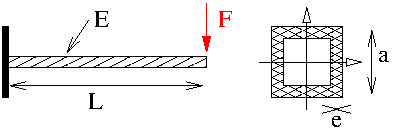
\includegraphics[width=10cm]{Figures/poutre.pdf}
  \end{center}
  \caption{cantilever beam under a ponctual bending load.}
\end{figure}


The objective of this study is to evaluate the influence of uncertainties of the input data $(E, F, L, I)$ on the deviation $y$.\\

We consider a steel beam with a hollow square section of length $a$ and of thickness $e$. Thus, the flexion section inertie of the beam is equal to $I = \displaystyle \frac{a^4 - (a-e)^4}{12}$. The beam length is $L$. The Young's modulus is $E$. The charge applied is $F$.\\

The  values used for the deterministic studies are :
\begin{align*}
  \left\{
  \begin{array}{lcl}
    E & = & 3.0e9 Pa\\
    F & = & 300 N\\
    L & = & 2.5m\\
    I & = & 4.0e-6 m^4.
  \end{array}
  \right.
\end{align*}

which corresponds to the point $(3.0e7, 30000, 250, 400)$ when the length $L$ is given in unit $cm$ et noo in the standard unit $m$.\\


This example treats the following points of the methodology :
\begin{itemize}
\item[$\bullet$] Min/Max approach : evaluation of the range of the output variable of interest (deviation)
  \begin{itemize}
  \item with a deterministic design of experiments ,
  \item with a random design of experiments ,
  \end{itemize}
\item[$\bullet$] Central tendancy approach : evaluation of the central indicators of the output variable of interest (deviation)
  \begin{itemize}
  \item Taylor variance decomposition,
  \item Random sampling,
  \item Kernel smoothing of the distribution of the output variable of interest,
  \end{itemize}
\item[$\bullet$] Threshold exceedance approach : evaluation of the probability that the output variable of interest (deviation) 30$\geq 30cm$
  \begin{itemize}
  \item FORM,
  \item Monte Carlo simulation method,
  \item Directional Sampling method,
  \item Importance Sampling method.
  \end{itemize}
\end{itemize}


\subsection{Probabilistic modelisation}

\subsubsection{Marginal distributions}

The random modelisation of the input data is the following one :
\begin{itemize}
\item[$\bullet$] E = Beta$(*)$ where $r = O.93,t = 3.2,a = 2.8e7,b = 4.8e7$,
\item[$\bullet$] F  = LogNormal, where the mean value is $E[F] = 30000$, the standard deviation is $\sqrt{\Var{F}} = 9000$ and the min value is $min(E) = 15000$,
\item[$\bullet$] L  = Uniform on $[250; 260]$,
\item[$\bullet$] I  = Beta$(*)$ where $r = 2.5,t = 4.0,a = 3.1e2,b = 4.5e2$.
\end{itemize}
(*) We recall here the expression of the probability density function of the Beta distribution :
\begin{align*}
  \displaystyle  p(x) = \frac{(x-a)^{(r-1)}(b-x)^{(t-r-1)}}{(b-a)^{(t-1)}B(r,t-r)}\boldsymbol{1}_{[a,b]}(x)
\end{align*}
where $r>0$, $t>r$ and $a < b$.



\subsubsection{Dependence structure}

We suppose that the probabilstic variables $L$ and $I$ are dependent. This dependence may be explained by the manufacturing process of the beam : the thiner the beam has been laminated, the longer it is.\\
We modelise the dependence structure by a Normal copula, parameterized from the Spearman correlation coefficient of both correlated variables : $\rho_S = -0.2$.\\
Then, the Spearman correlation matrix of the input random vector $(E,F,L,I)$ is :
\begin{align*}
  R_S = \left (
  \begin{array}{cccc}
    1 & 0 & 0 & 0 \\
    0 & 1 & 0 & 0 \\
    0 & 0 & 1 & -0.2 \\
    0 & 0 & -0.2 & 1
  \end{array}
  \right)
\end{align*}





\subsection{Min/Max approach}


\subsubsection{Deterministic design of experiments }

We consider a composite design of experiments , where :
\begin{itemize}
\item the levels of the centered and reducted grid are +/-0.5, +/-1., +/-3.,
\item the unit per dimension (scaling factor) is given by the standard deviation of the marginal distribution of the corresponding variable,
\item the center is the mean point of the input random vector distribution.
\end{itemize}



\subsubsection{Random sampling}

We evaluate the range of the deviation from a random sample of size $10^4$.



\subsection{Central tendancy approach}


\subsubsection{Taylor variance decomposition}

We evaluate the mean and the standard deviation of the deviation thanks to the Taylor variance decomposition method. The importance factors of that method rank the influence of the input uncertainties on the mean of the deviation.

\subsubsection{Random sampling}

We evaluate the mean and standard deviation of the deviation from a random sample of size $10^4$.

\subsubsection{Kernel smoothing}

We fit the distribution of the deviation with a Normal kernel, which bandwidth is evaluated from the Scott rule, from a random sample of size $10^4$.\\
We superpose then the kernel smoothing pdf and the normal one which mean and standard deviation are those of the random sample of the output variable of interest in order to graphically check if the Normal model fits to the deviation distribution.

\subsection{Threshold exceedance approach}

We consider the event where the deviation exceeds $30 cm$.\\

\subsubsection{FORM}

We use the Cobyla algorithm to research the design point, which requires no evaluation of the gradient of the limit state function. We parameterize the Cobyla algorithmwit hte following parameters :
\begin{itemize}
\item Maximum Iterations Number = $10^3$,
\item Maximum Absolute Error = $10^{-10}$,
\item Maximum Relative Error = $10^{-10}$,
\item Maximum Residual Error = $10^{-10}$,
\item Maximum Constraint Error = $10^{-10}$.
\end{itemize}


\subsubsection{Monte Carlo simulation method}

We evaluate the probability with the Monte Carlo method, parameterized as follows :
\begin{itemize}
\item Maximum Outer Sampling = $4\, 10^4$,
\item Block Size = $10^2$,
\item Maximum Coefficient of Variation = $10^{-1}$.
\end{itemize}

We evaluate the confidence interval of level $0.95$ and we draw the convergence graph of the Monte Carlo estimator with its confidence interval of level 0.90.



\subsubsection{Directional Sampling method}

We evaluate the probability with the Directional Sampling method, with its default parameters :
\begin{itemize}
\item 'Slow and Safe' for the root strategy,
\item 'Random direction' for the sampling strategy
\end{itemize}


We evaluate the confidence interval of level $0.95$ and we draw the convergence graph of the Directional Sampling  estimator with its confidence interval of level 0.90.


\subsubsection{Importance Sampling method}


We evaluate the probability with the Importance Sampling method in the standard sapce, with the same parameters as the Monte carlo method. The importance distribution is the normal one, centered on the standard design point and which standard deviation is 4. The importance sampling is performed in the standard sapce.\\

We fix the BlockSize is fixed to 1 and the MaximumOuterIteration to $4\, 10^4$.\\

We draw the convergence graph of the Importance Sampling  estimator with its confidence interval of level 0.90.




\subsection{Response surface by polynomial chaos expansion}


We evaluate the meta model determined thanks to the polynomial chaos expansion technique.




We took the following 1D polynomial families, which parameters have been determined in order to be adapted to the marginal distributions of the input random vector :
\begin{itemize}
\item $E$ : Jacobi($\alpha = 1.3$, $\beta = -0.1$, \textit{param}=Jacobi.ANALYSIS),
\item $F$ : Laguerre($k = 1.78$, Laguerre.ANALYSIS),
\item $L$ : Legendre,
\item $I$ : Jacobi($\alpha = 0.5$, $\beta = 1.5$, \textit{param}=Jacobi.ANALYSIS).
\end{itemize}

The truncature strategy of the multivariate orthonormal basis is the Cleaning Strategy where we considered within the $500$ first terms of the multivariate basis, among the 50 most significant ones, those which contribution wre significant (which means superior to $10^{-4}$).\\

The evaluation strategy of the approximation coefficients is the least square strategy based on a design of experiments  determined with the Monte Carlo sampling technique of size 100.\\

Figures (\ref{PCE_E}) to (\ref{ModelsComparison}) draw the following graphs :
\begin{itemize}
\item the drawings of some members of the 1D polynomial family,
\item the cloud of points making the comparison between the model values and the meta model ones : if the adequation is perfect, points must be on the first diagonal.
\end{itemize}















%%%%%%%%%%%%%%%%%%%%%%%%%%%%%%%%%%%%%
\subsection{The Python script}


\lstset{language=python, keywordstyle=\color{black}\bfseries,tabsize=2,framexleftmargin=8mm,frame=shadowbox,rulesepcolor=\color{black},numbers=left,breaklines=true}

\lstinputlisting{scriptExample_beam.py}




%%%%%%%%%%%%%%%%%%%%%%%%%%%%%%%%%%%%%
\subsection{Output of the Python script}

\lstinputlisting{resultatExampleBeam}



%%%%%%%%%%%%%%%%%%%%%%%%%%%%%%%%%%%%%
\subsection{Figures}


The probability density function (PDF) of each marginal is given in Figures \ref{pdfE} to \ref{pdfI}.


\begin{figure}[Hhbtp]
  \begin{minipage}{9.8cm}
    \begin{center}
      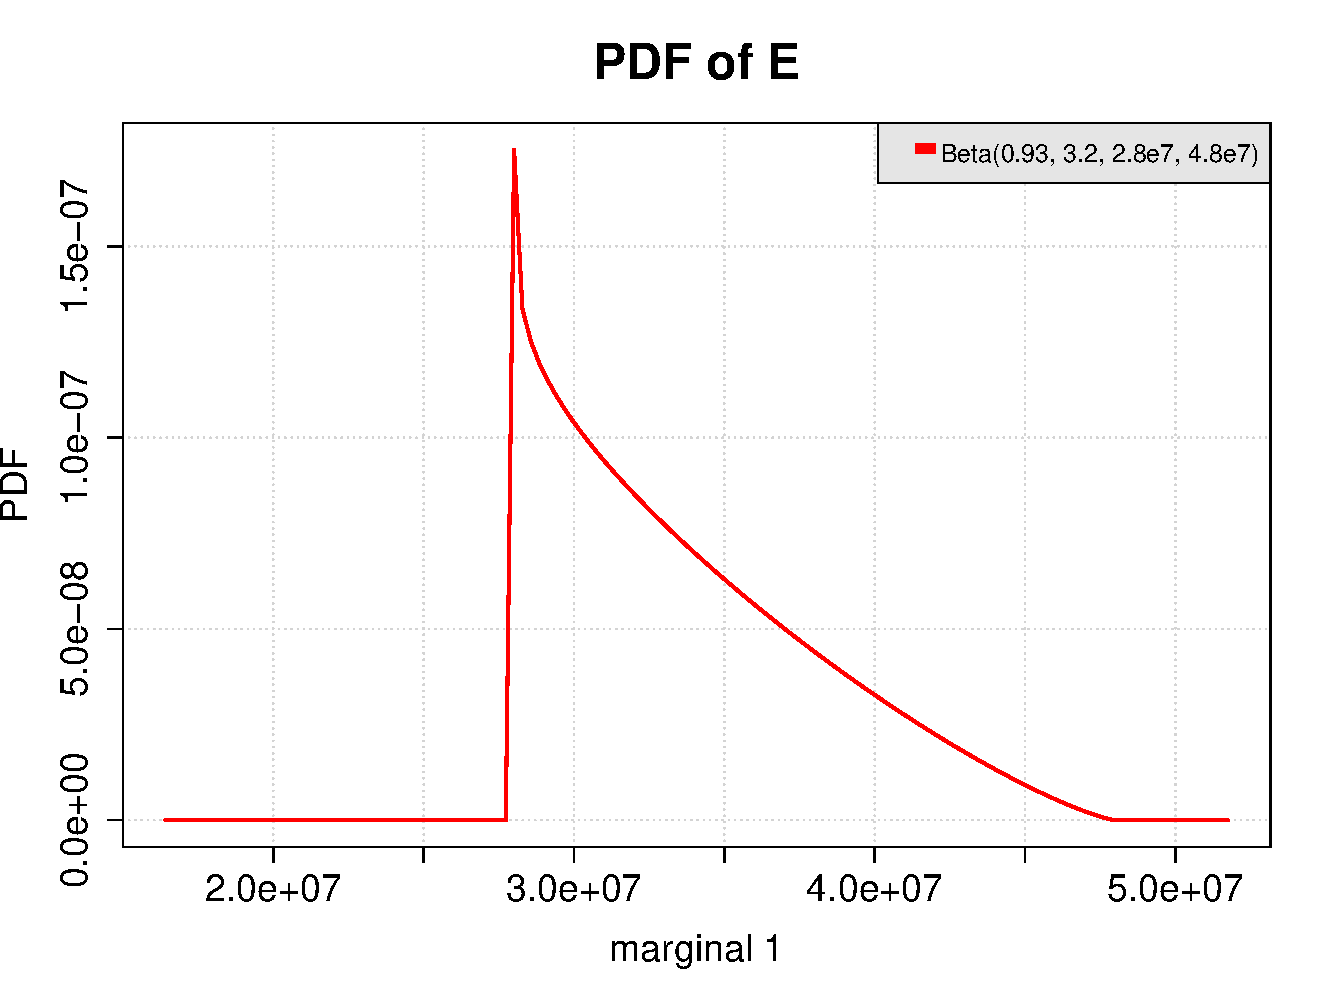
\includegraphics[width=7cm]{Figures/distributionE_pdf.pdf}
      \caption{Probability density function of the parameter E}
      \label{pdfE}
    \end{center}
  \end{minipage}
  \hfill
  \begin{minipage}{9.8cm}
    \begin{center}
      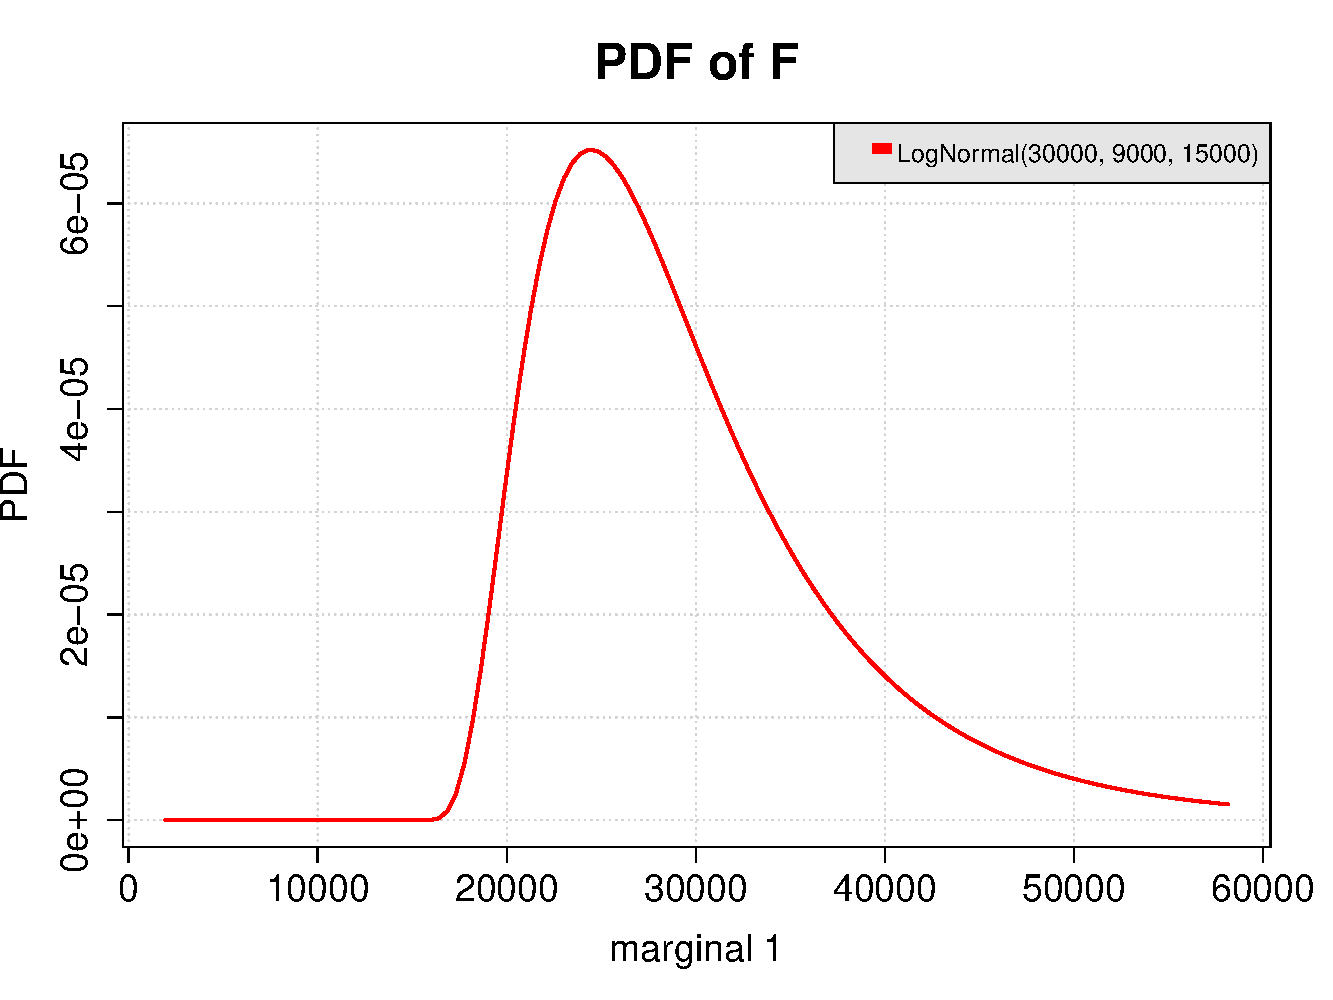
\includegraphics[width=7cm]{Figures/distributionF_pdf.pdf}
      \caption{Probability density function of the parameter F}
      \label{pdfF}
    \end{center}
  \end{minipage}
\end{figure}


\begin{figure}[Hhbtp]
  \begin{minipage}{9.8cm}
    \begin{center}
      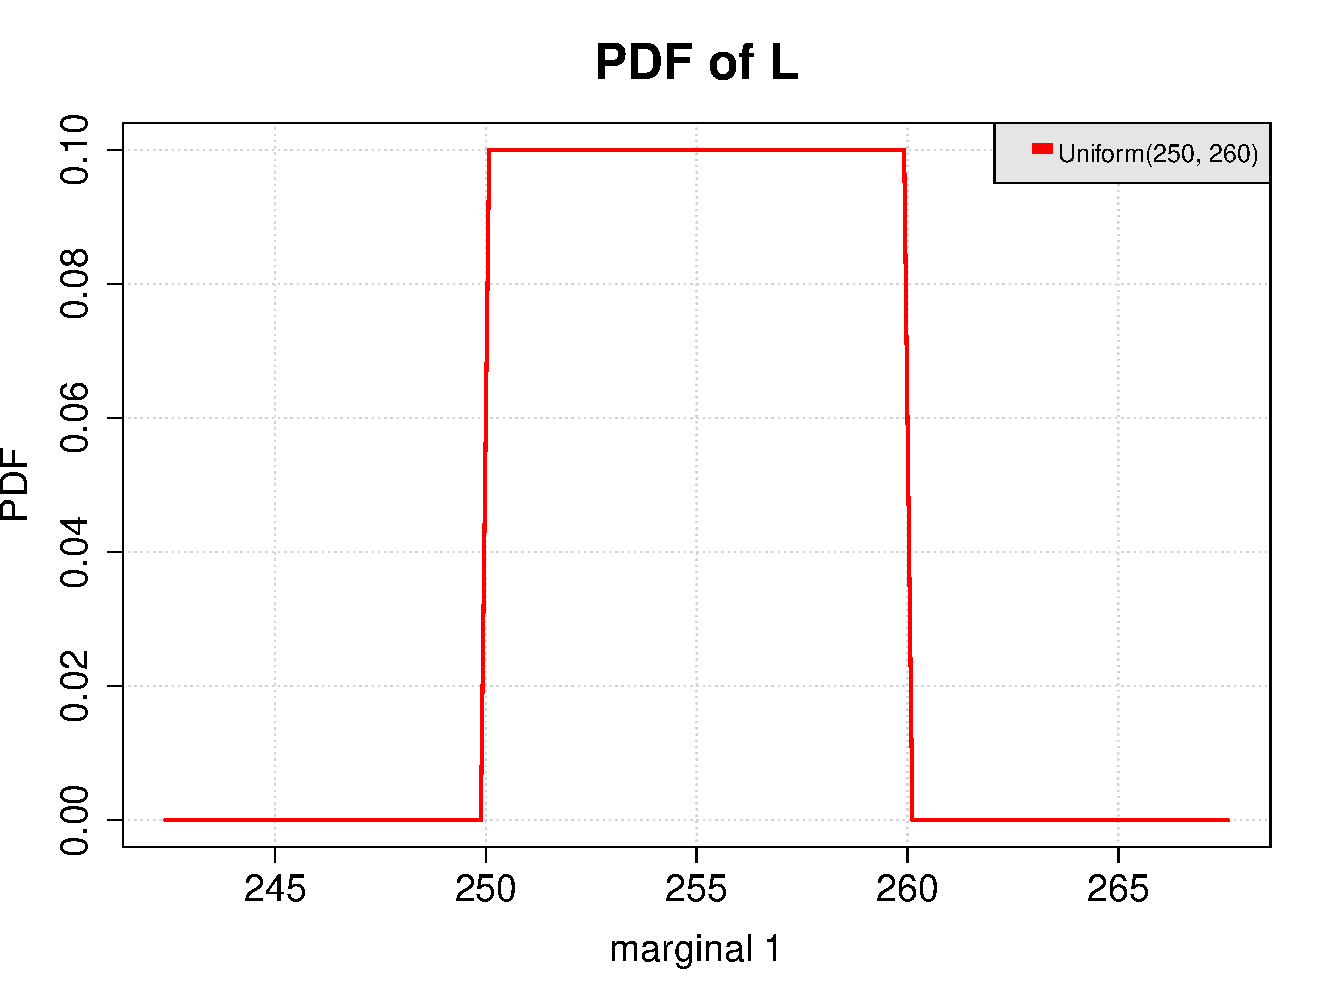
\includegraphics[width=7cm]{Figures/distributionL_pdf.pdf}
      \caption{PDFof the parameter L}
      \label{pdfL}
    \end{center}
  \end{minipage}
  \hfill
  \begin{minipage}{9.8cm}
    \begin{center}
      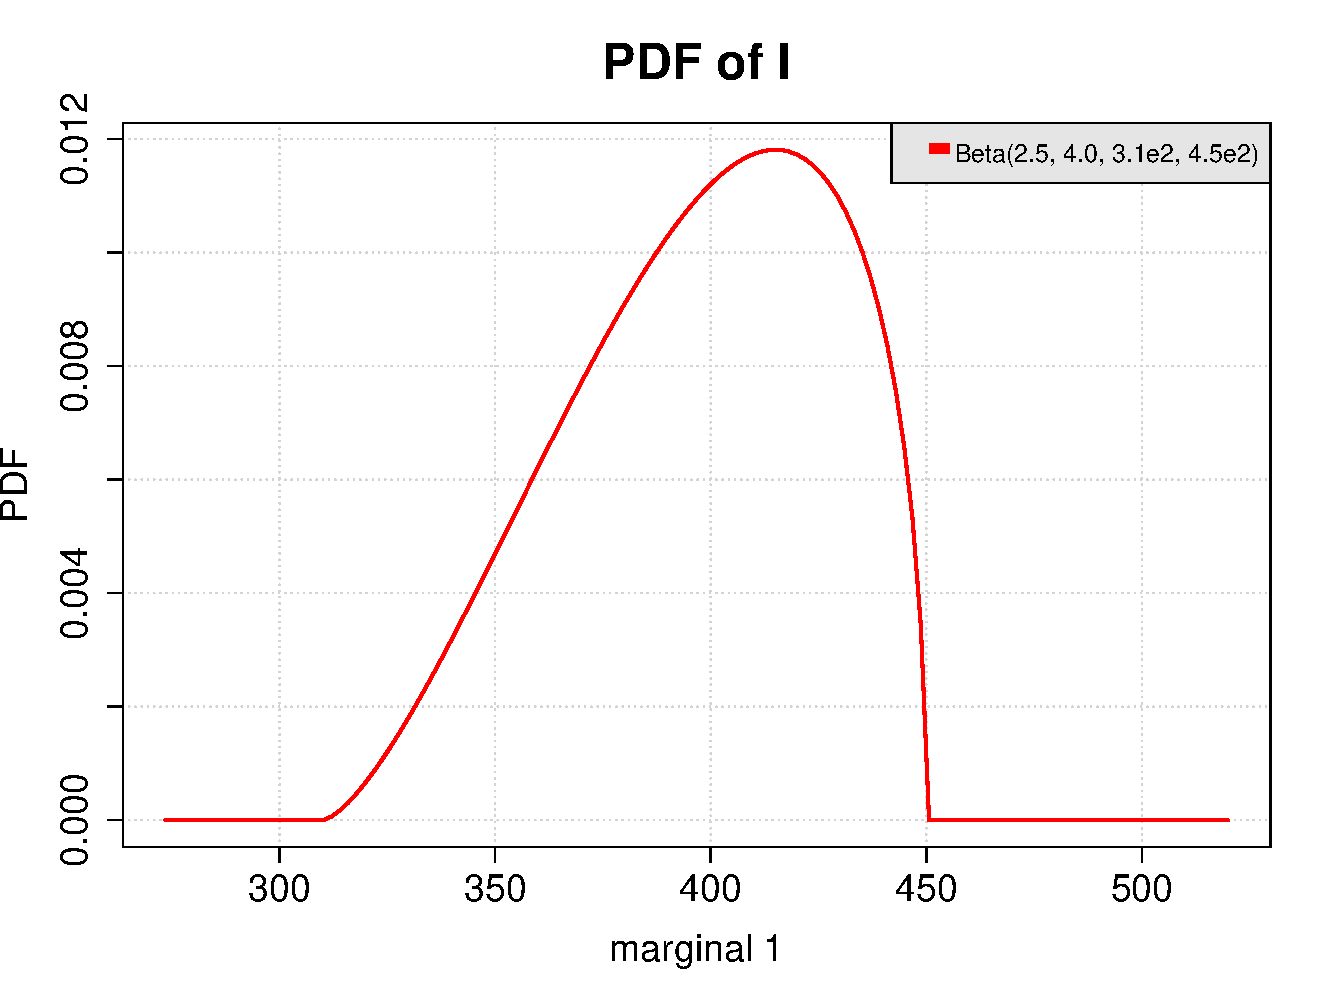
\includegraphics[width=7cm]{Figures/distributionI_pdf.pdf}
      \caption{PDF of the parameter I}
      \label{pdfI}
    \end{center}
  \end{minipage}
\end{figure}

The probability density function (PDF) and the cumulative density function (CDF) of the deviation fiited with the kernel smoothing metid are drawn in Figures \ref{KernelSmoothing} and  \ref{KernelSmoothing2}.



\begin{figure}[Hhbtp]
  \begin{minipage}{9.8cm}
    \begin{center}
      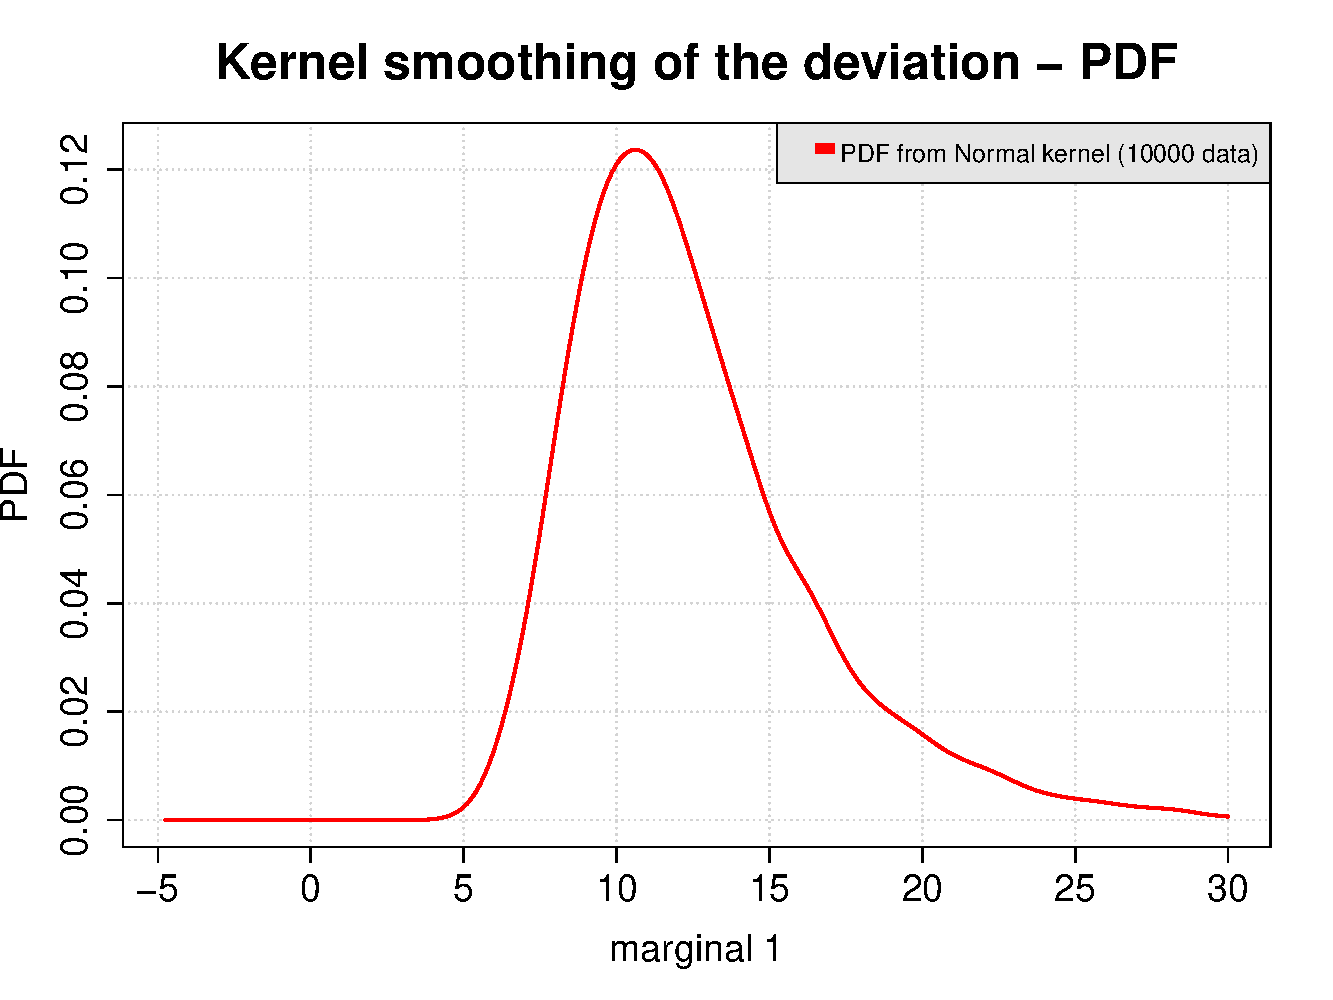
\includegraphics[width=7cm]{Figures/smoothedPDF.pdf}
      \caption{PDF of the deviation with the kernel smoothing method.}
      \label{KernelSmoothing}
    \end{center}
  \end{minipage}
  \hfill
  \begin{minipage}{9.8cm}
    \begin{center}
      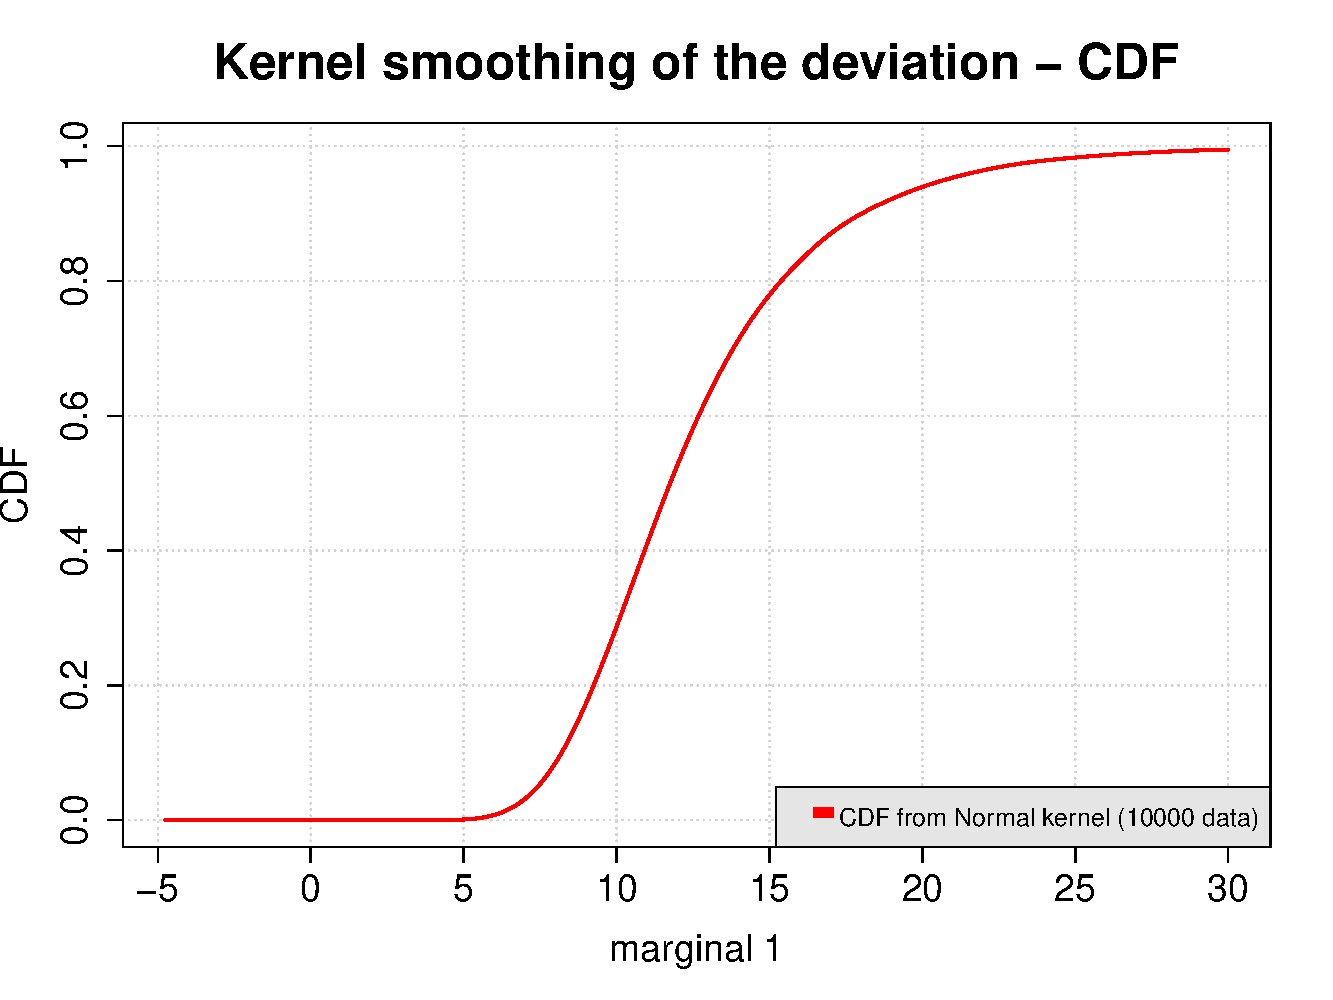
\includegraphics[width=7cm]{Figures/smoothedCDF.pdf}
      \caption{CDF of the deviation with the kernel smoothing method.}
      \label{KernelSmoothing2}
    \end{center}
  \end{minipage}
\end{figure}


The superposition of the kernel smoothed density function and the normal fitted from the same sample with the maximum likelihood method is drawn in Figure \ref{superp}.


\begin{figure}[Hhbtp]
  \begin{center}
    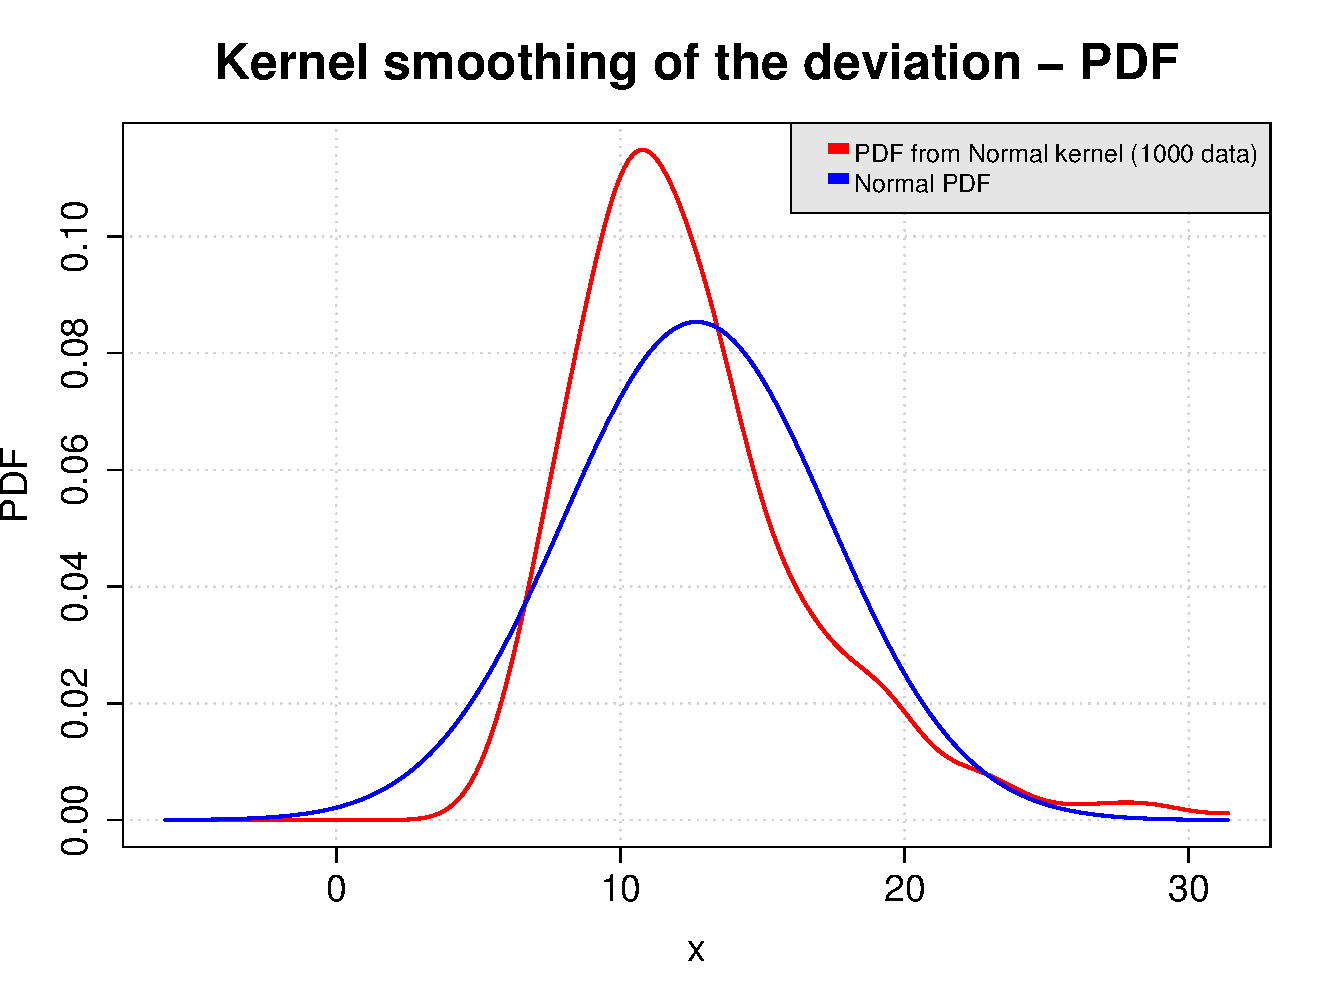
\includegraphics[width=9cm]{Figures/smoothedPDF_and_GaussianPDF.pdf}
  \end{center}
  \caption{Superposition of the kernel smoothed density function and the normal fitted from the same sample.}
  \label{superp}
\end{figure}

The importance factors from the FORM method are given in Figure \ref{FormIF}.

\begin{figure}[Hhbtp]
  \begin{center}
    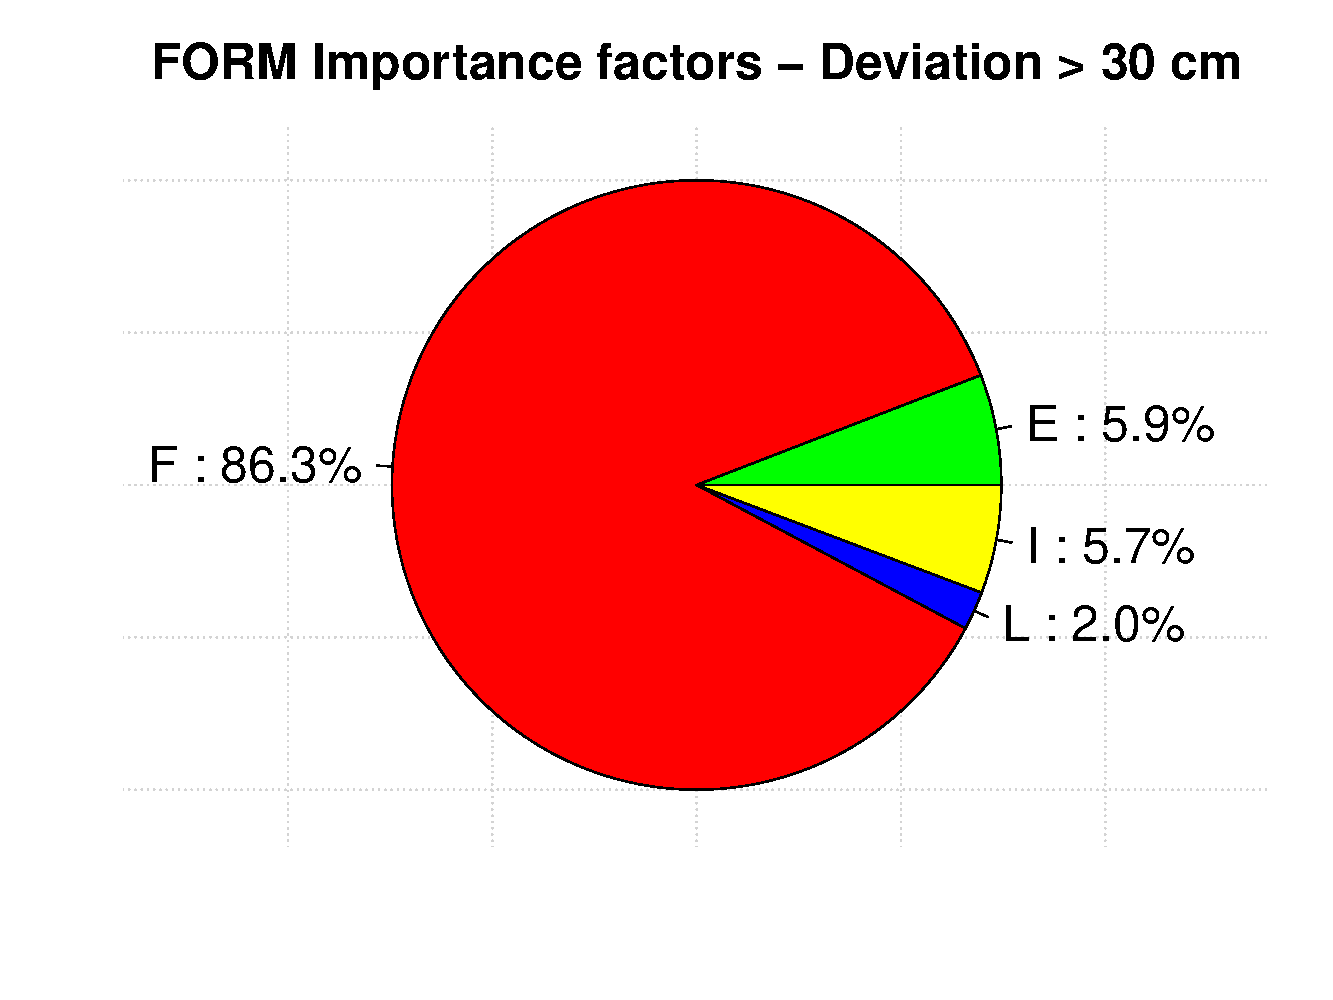
\includegraphics[width=9cm]{Figures/ImportanceFactorsDrawingFORM.pdf}
  \end{center}
  \caption{FORM importance factors of the event : deviation > 30 cm.}
  \label{FormIF}
\end{figure}

The convergence graphs of the simulation methods are given in Figures \ref{MCConvergence} to \ref{ISConvergence}.


\begin{figure}[Hhbtp]
  \begin{minipage}{9.8cm}
    \begin{center}
      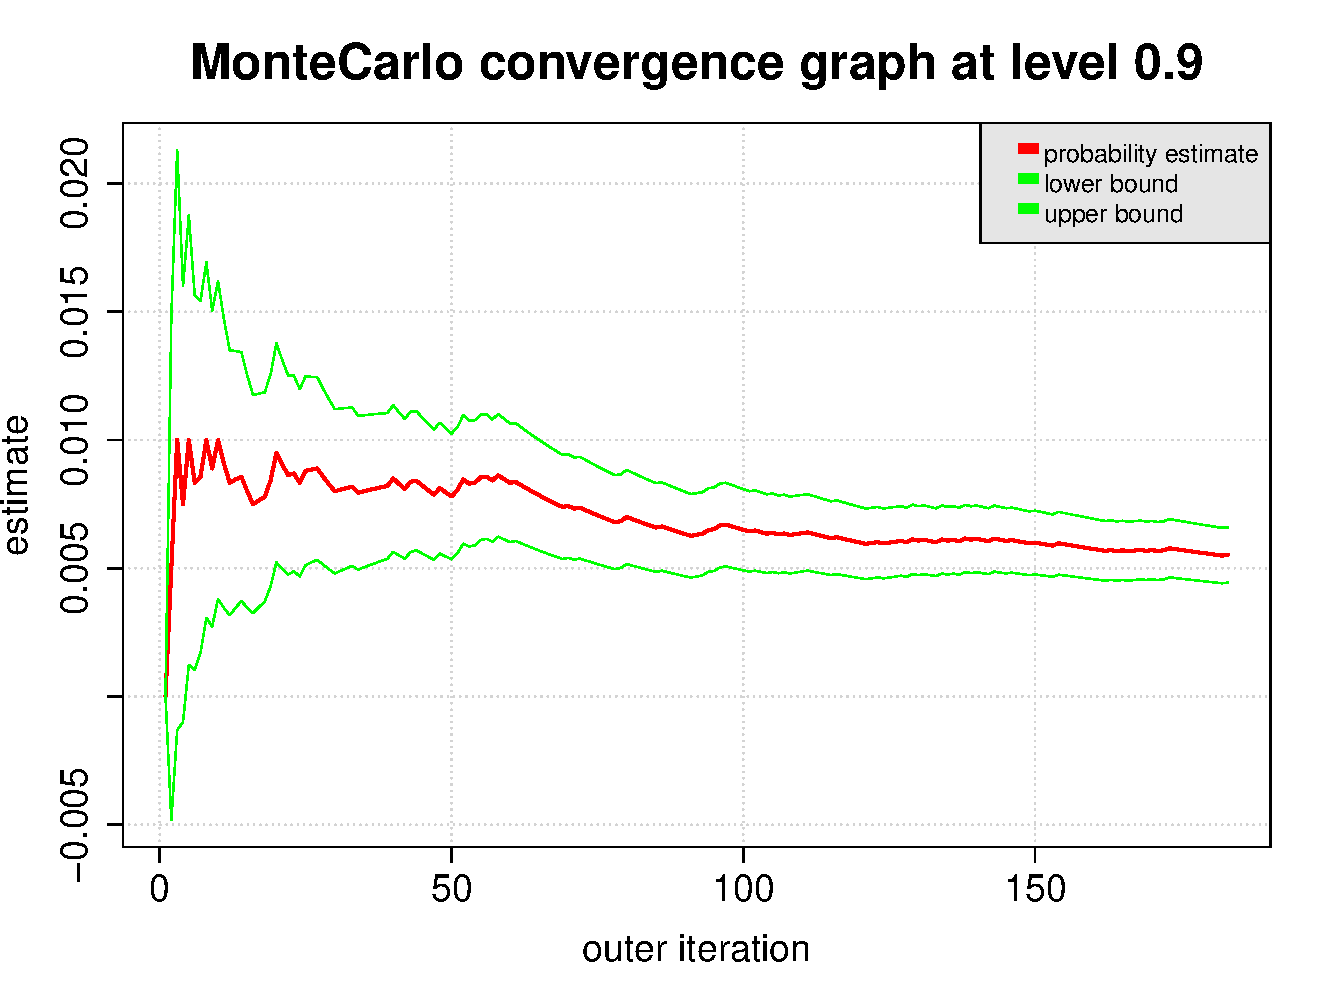
\includegraphics[width=7cm]{Figures/convergenceGrapheMonteCarlo.pdf}
      \caption{Monte Carlo convergence graph.}
      \label{MCConvergence}
    \end{center}
  \end{minipage}
  \hfill
  \begin{minipage}{9.8cm}
    \begin{center}
      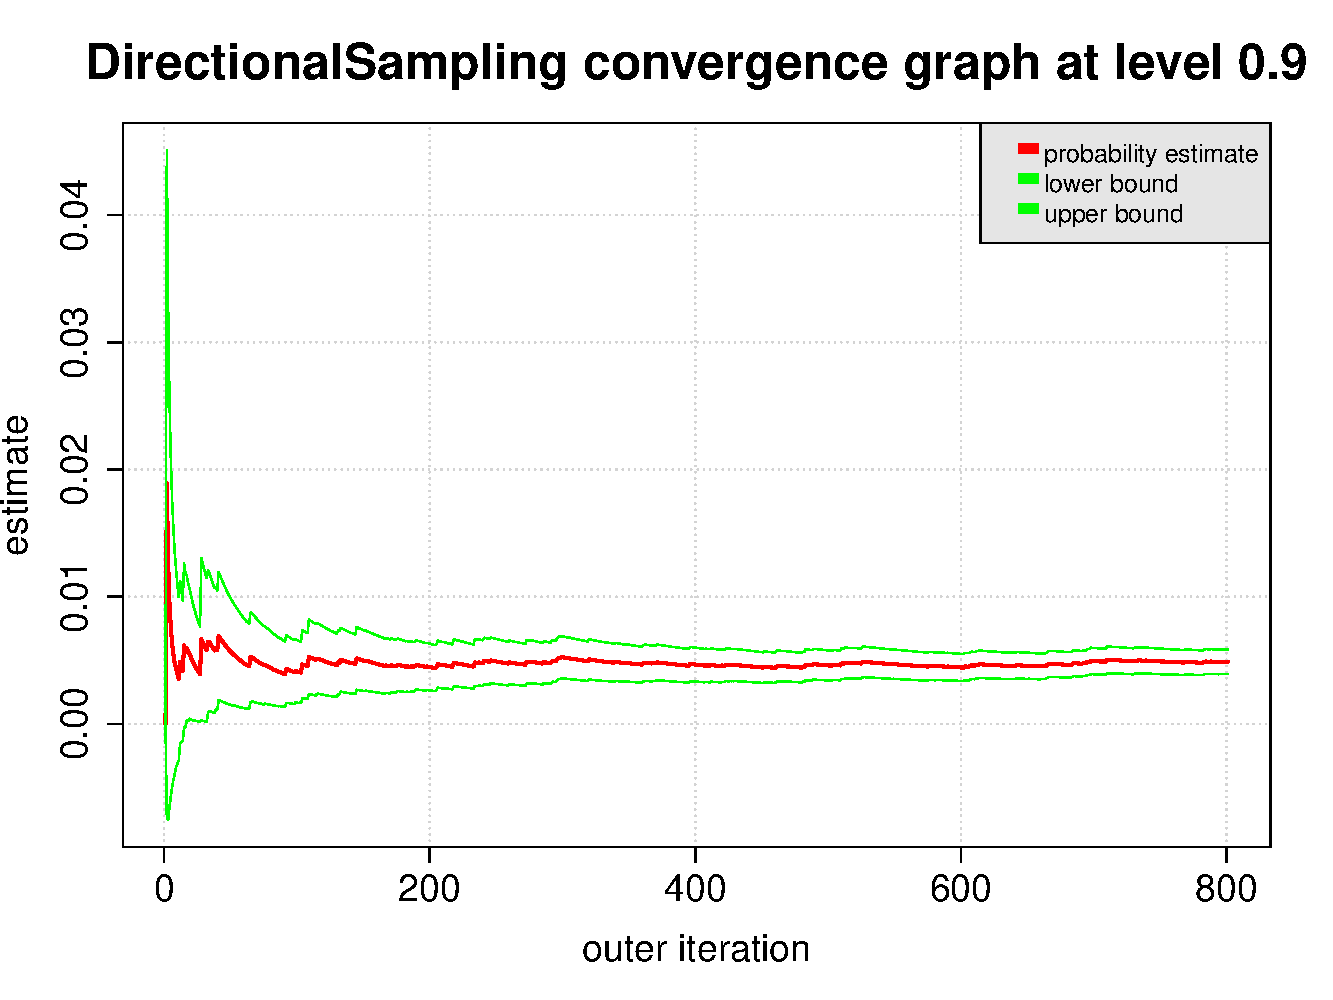
\includegraphics[width=7cm]{Figures/convergenceGrapheDS.pdf}
      \caption{Directional Sampling convergence graph.}
      \label{DSConvergence}
    \end{center}
  \end{minipage}
\end{figure}




\begin{figure}[Hhbtp]
  \begin{minipage}{9.8cm}
    \begin{center}
      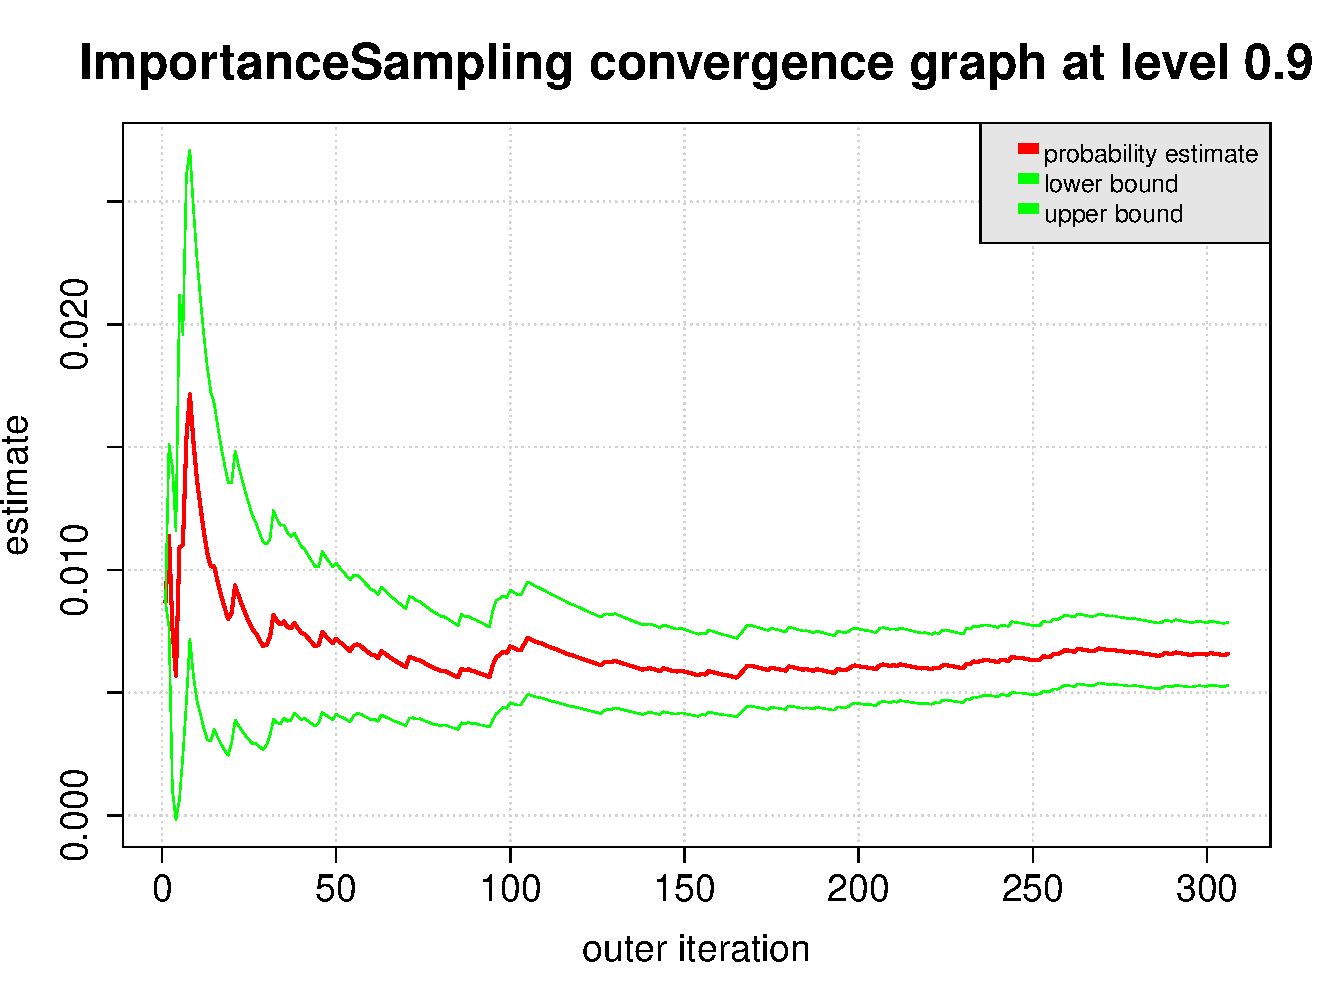
\includegraphics[width=7cm]{Figures/convergenceGrapheIS.pdf}
      \caption{Importance sampling convergence graph.}
      \label{ISConvergence}
    \end{center}
  \end{minipage}
\end{figure}


Figures (\ref{PCE_E}) to (\ref{ModelsComparison}) contain the graphs :

\begin{itemize}
\item Graph 1 : the drawings of the fith first members of the 1D polynomial family,
\item Graph 2 : the cloud of points making the comparison between the model values and the meta model ones : if the adequation is perfect, points must be on the first diagonal.
\end{itemize}


\begin{figure}[Hhbtp]
  \begin{minipage}{9cm}
    \begin{center}
      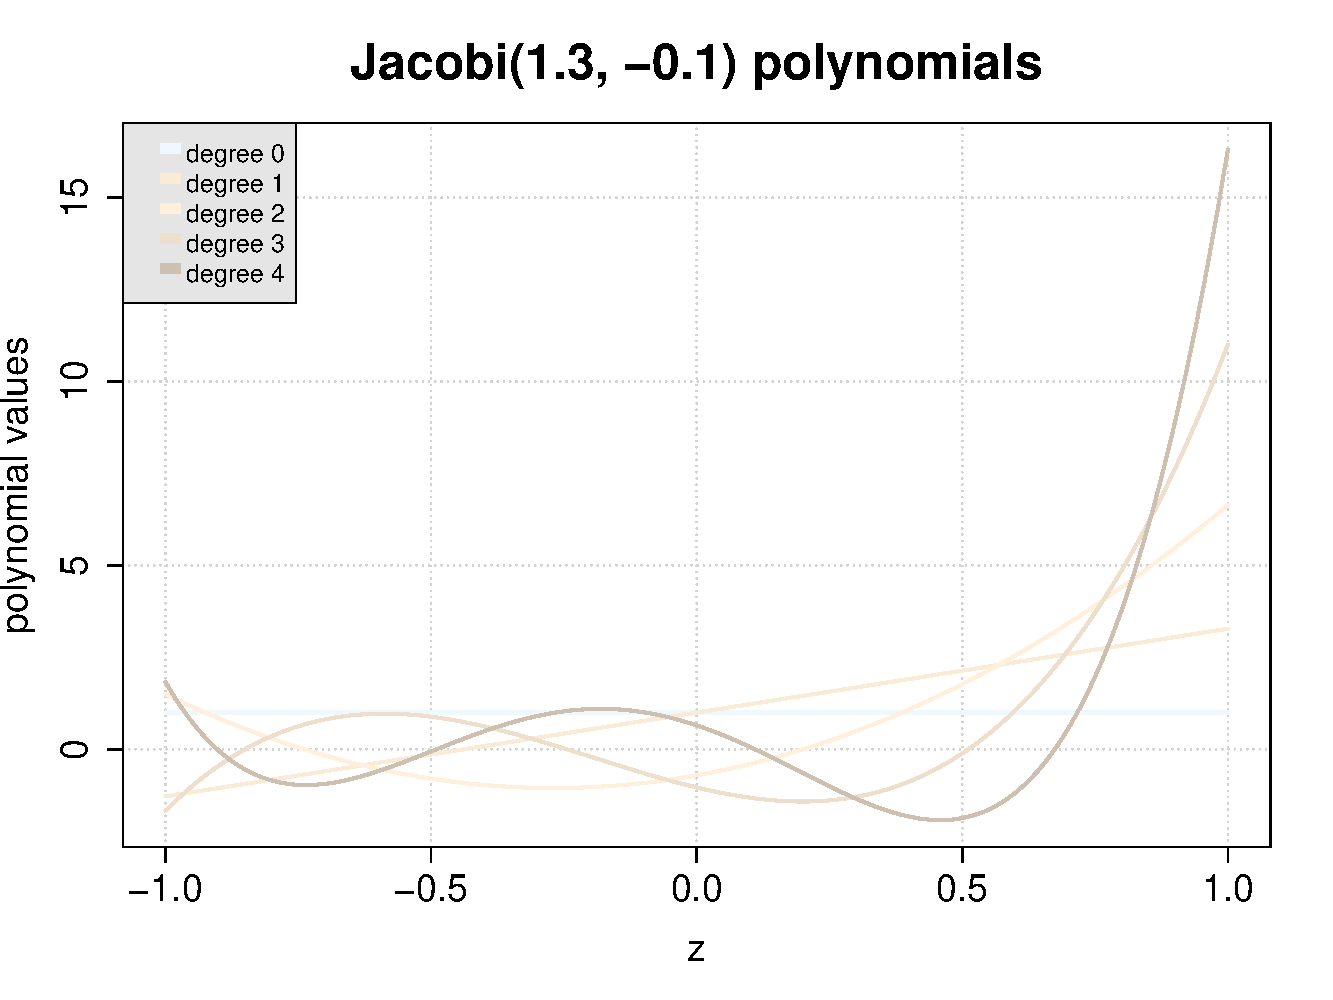
\includegraphics[width=7cm]{Figures/PCE_JacobiPolynomials_VariableE.pdf}
      \caption{The 5-th first polynomials of the Jacobi family associated to the variable $E$.}
      \label{PCE_E}
    \end{center}
  \end{minipage}
  \hfill
  \begin{minipage}{9cm}
    \begin{center}
      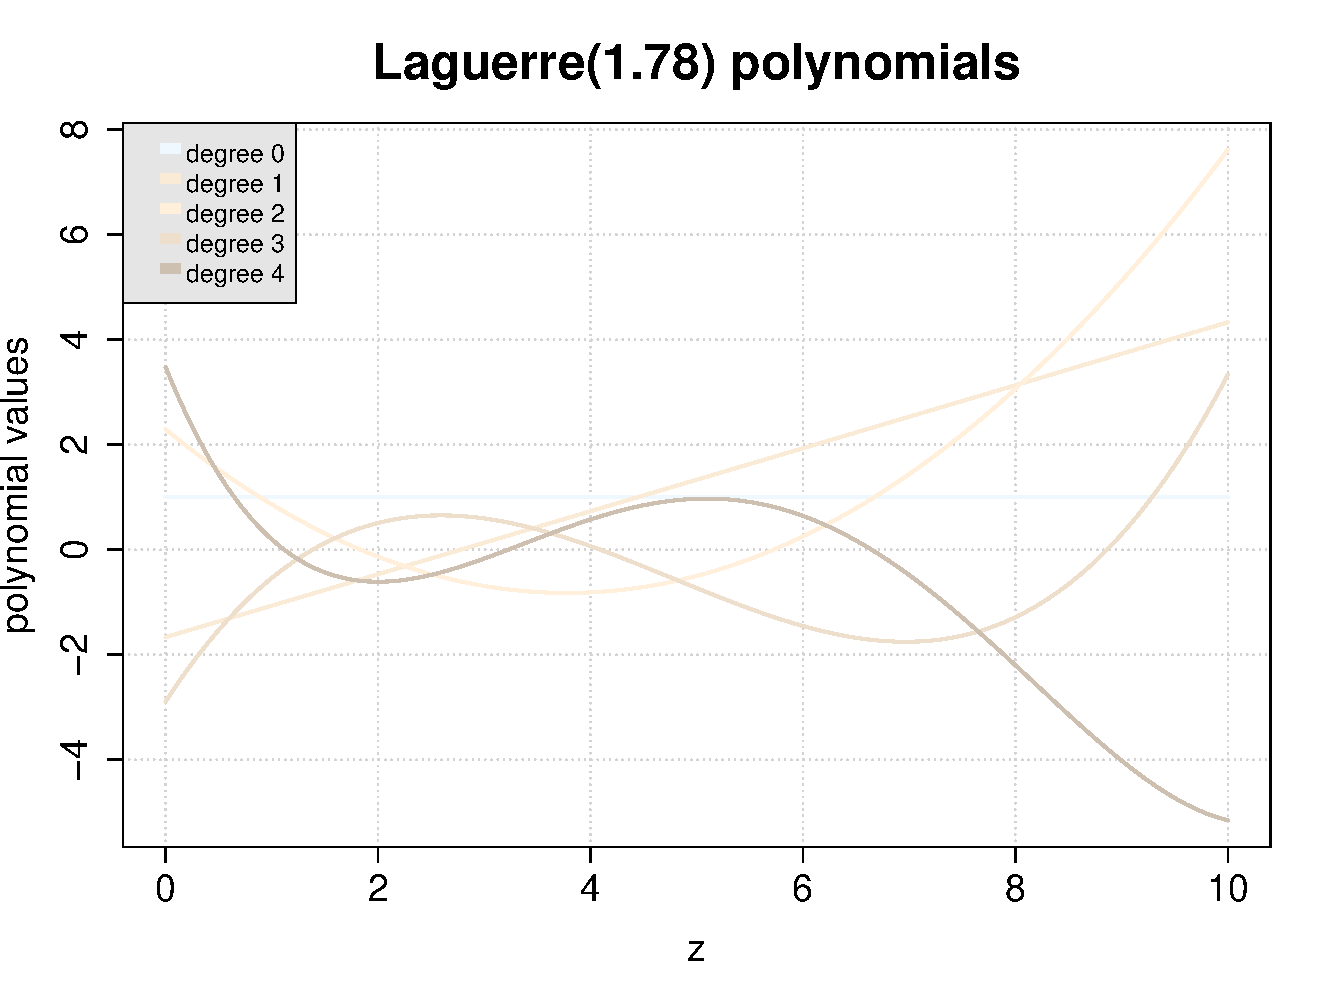
\includegraphics[width=7cm]{Figures/PCE_LaguerrePolynomials_VariableF.pdf}
      \caption{The 5-th first polynomials of the Laguerre family associated to the variable $F$.}
      \label{PCE_F}
    \end{center}
  \end{minipage}
\end{figure}

\begin{figure}[Hhbtp]
  \begin{minipage}{9cm}
    \begin{center}
      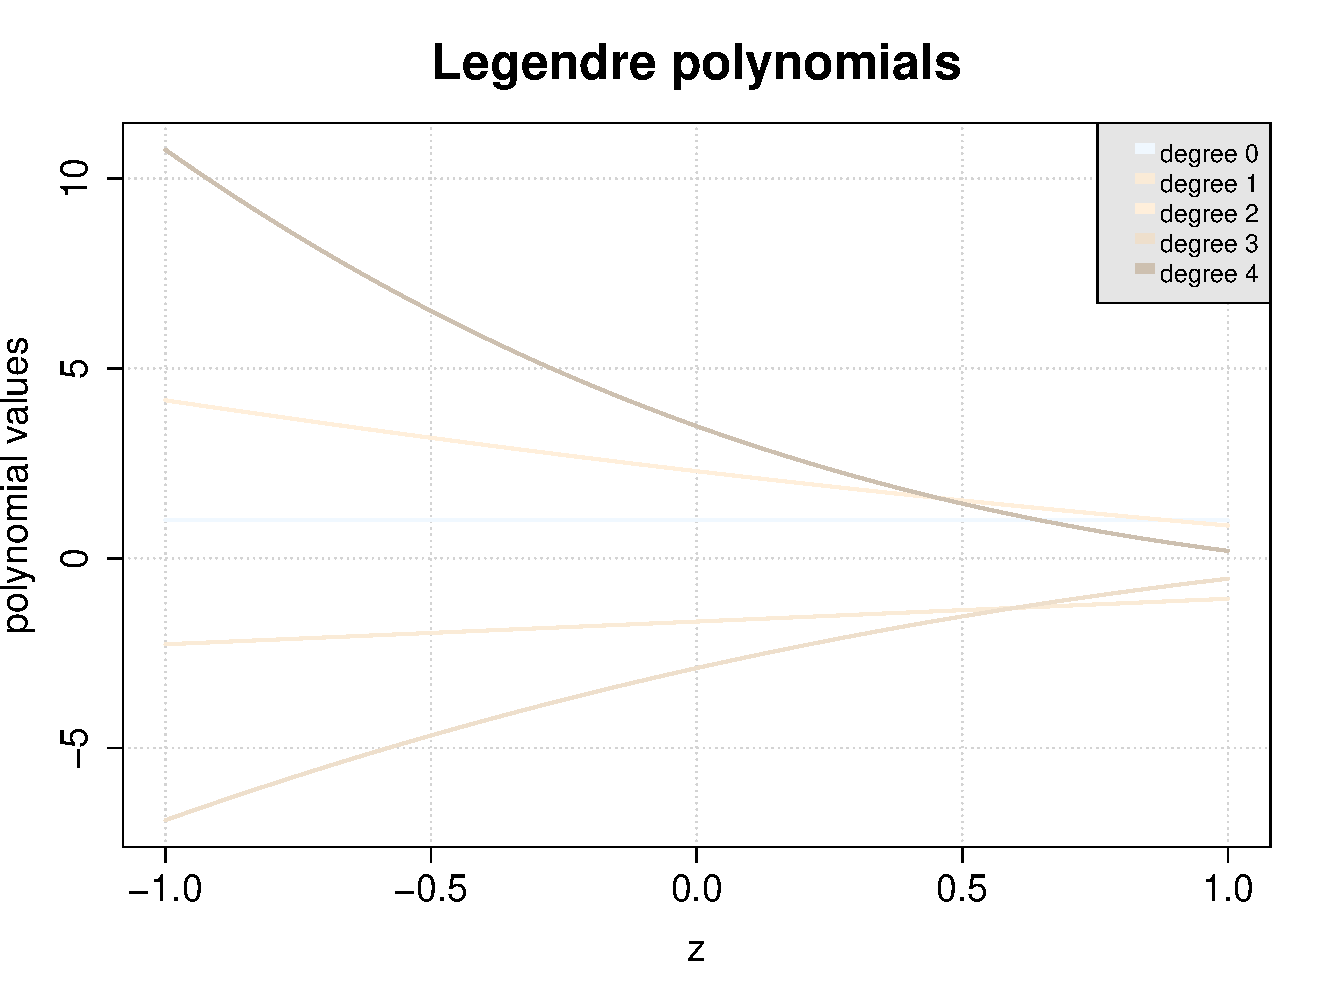
\includegraphics[width=7cm]{Figures/PCE_LegendrePolynomials_VariableL.pdf}
      \caption{The 5-th first polynomials of the Legendre associated to the variable $L$.}
      \label{PCE_L}
    \end{center}
  \end{minipage}
  \hfill
  \begin{minipage}{9cm}
    \begin{center}
      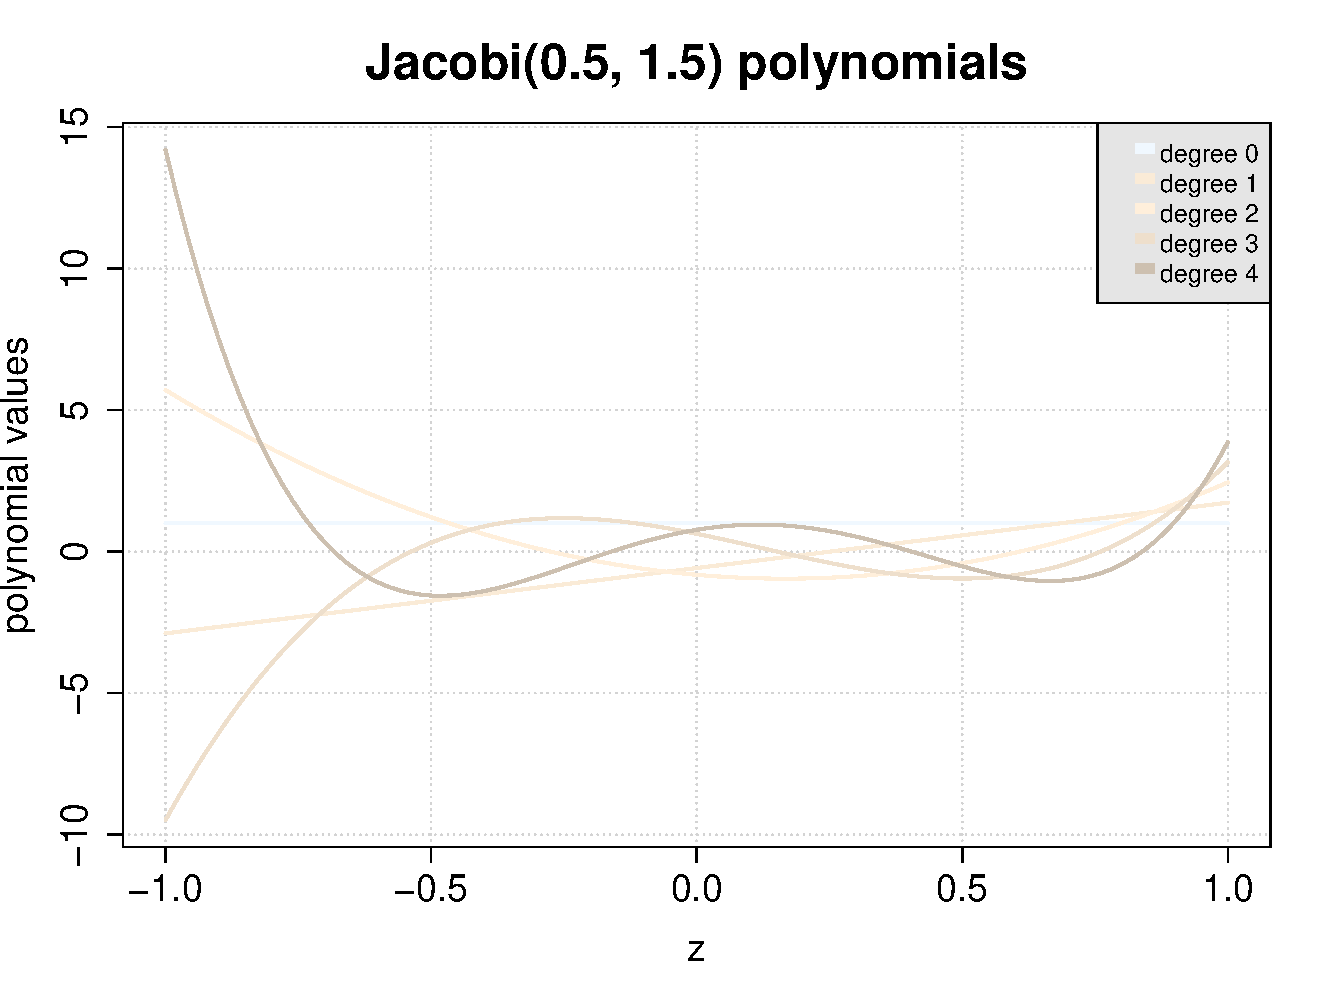
\includegraphics[width=7cm]{Figures/PCE_JacobiPolynomials_VariableI.pdf}
      \caption{The 5-th first polynomials of the Jacobi family associated to the variable $I$.}
      \label{PCE_I}
    \end{center}
  \end{minipage}
\end{figure}




\begin{figure}[Hhbtp]
  \begin{center}
    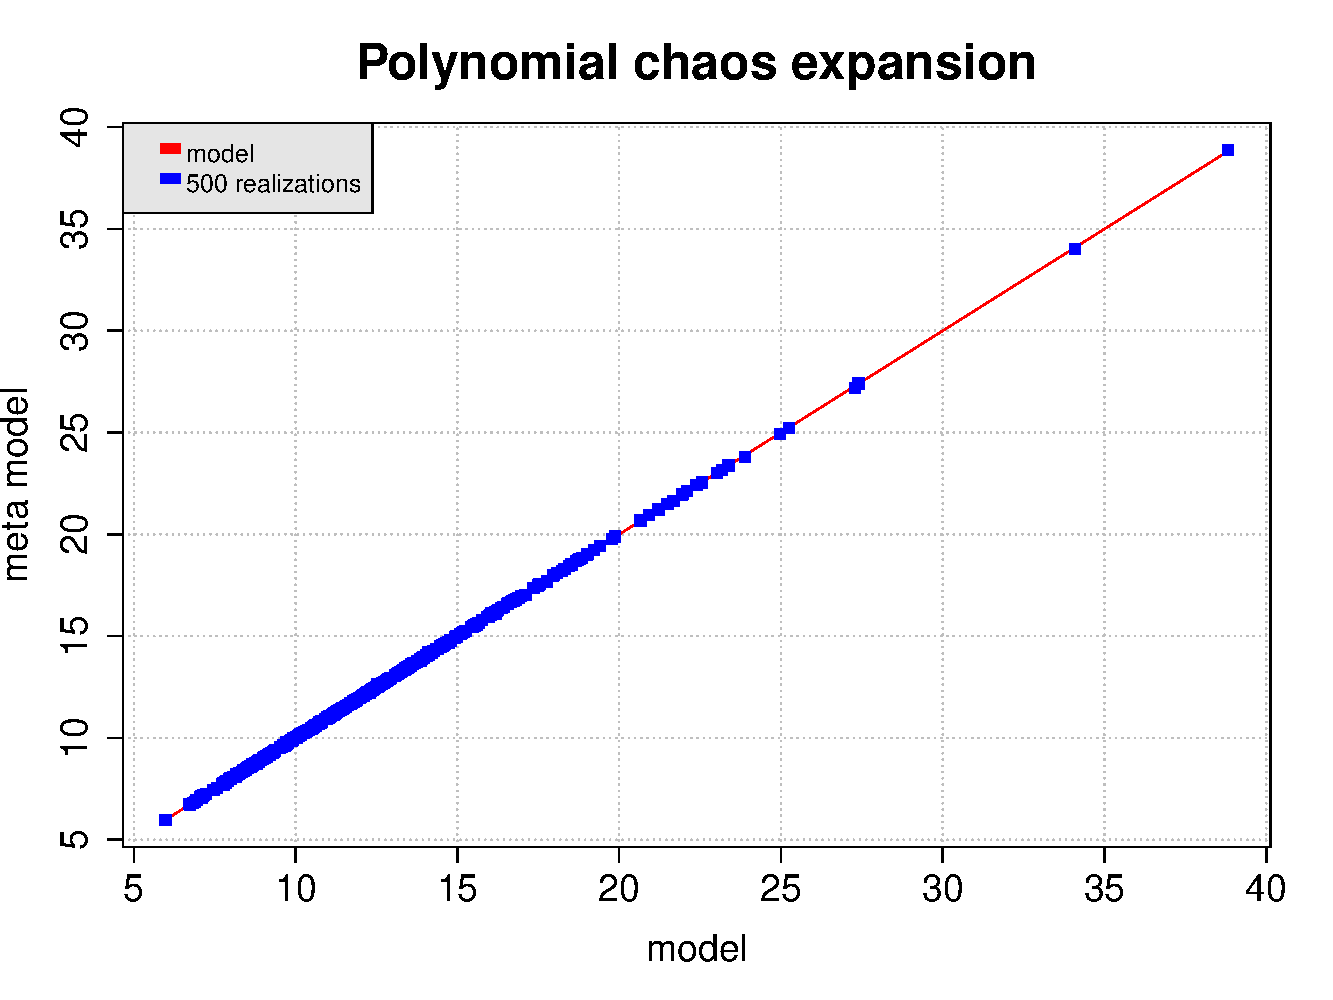
\includegraphics[width=7cm]{Figures/PCE_comparisonModels.pdf}
    \caption{Comparison of values from the model and the polynomial chaos meta model.}
    \label{ModelsComparison}
  \end{center}
\end{figure}




\subsection{Results comments}

\subsubsection{Min/Max approach}

The Min/Max approach enables to evaluate the range of the deviation.\\

We note that the use of an design of experiments  may be benefical with regard the random sampling technique as we can catch more easily (which means with less evaluations of the limit state function) the extrem values of the output variable of interest :h ere, we have managed to catch both extrem bounds of the deviation with the composite design of experiments , whereas the random sampling technique did not manage to give a good evaluation of them.\\

Note that the composite design of experiments  has 73 points, where as the random sampling technique has been effected with $10^4$ points.



\subsubsection{Central tendancy approach}

The Taylor variance decomposition has given a good approximation of  the mean value of the deviation : the value is comparable to the one obtained with the random technique. Furthermore, note that the Taylor variance decomposition required only 1 evaluation of the limit state function, whereas the random sampling technique required $10^4$ evaluations.\\

The second order evaluation of the mean by the  Taylor variance decomposition method adds no information, which probably means that around the mean point of the input random vector, the limit state function is well approximated by its tangent plane.\\

The importance factors indicate that the mean of the deviation is mostly influenced by the uncertainty of the variable $F$.\\

The kernel smoothing technique enables to have a look on the distribution shape and  another approximation of the mean value of the deviation.\\
Note that the normal fitting on the sample is not adapted.



\subsubsection{Threshold exceedance approach}

The whole event probabilities evaluated from the simulation methods are equivalent and confirm the event probability evaluated with FORM.\\

Note that the FORM probability required only 194 evaluations of the limit state function whereas the Monte Carlo probability required 18300 evaluations and the Directional Sampling one 14378 evaluations.\\
The Importance Sampling is a simulation method but the importance density has been centered around the design point, where the threshold exceedance is concentrated. That's why the succession of the FORM technique and the Importance sampling one where the importance density is a normal distribution centered around the design point, performed in the standard space, seems to be the better compromise between the limit state evaluation calls number and the probability evaluation precision.\\

The simulation methods give a confidence interval, which is not possible with FORM.\\

FORM ranks the influence of the input uncertainties on the realization of the threshold exceedance event : the variable $F$ is largely the more influent. Thus, if the threshold exceedance probability is judged too high, it is recommanded to decrease the variability of the variable $F$ first.


\subsubsection{Response surface : Polynomial expansion chaos}

The polynomial expansion chaos has defined a meta model thanks to 10000 points, which gives very satisfactory results compared to those obtained with other methods.




% -------------------------------------------------------------------------------------------------
\newpage
\section{Example 2: elastic truss structure}

\subsection{Problem statement}

\subsubsection{Physical model}

Let us consider the elastic truss structure represented in Figure~\ref{fig_treillis}. The structure comprises three bars (labelled 1,2 and 3) with specific cross-section areas and Young's moduli (denoted by $S_1$, $S_2$, $S_3$ and $E_1$, $E_2$, $E_3$, respectively). The angle between bar \#1 and bar \#3 (resp. bar \#2 and bar \#3) is denoted by $\alpha_1$ (resp. $\alpha_2$). The system is subjected to an oblical point load $P$ such that the angle between $P$ and bar \#3 is equal to $\theta$.

\begin{figure}[Hhbtp]
  \begin{center}
    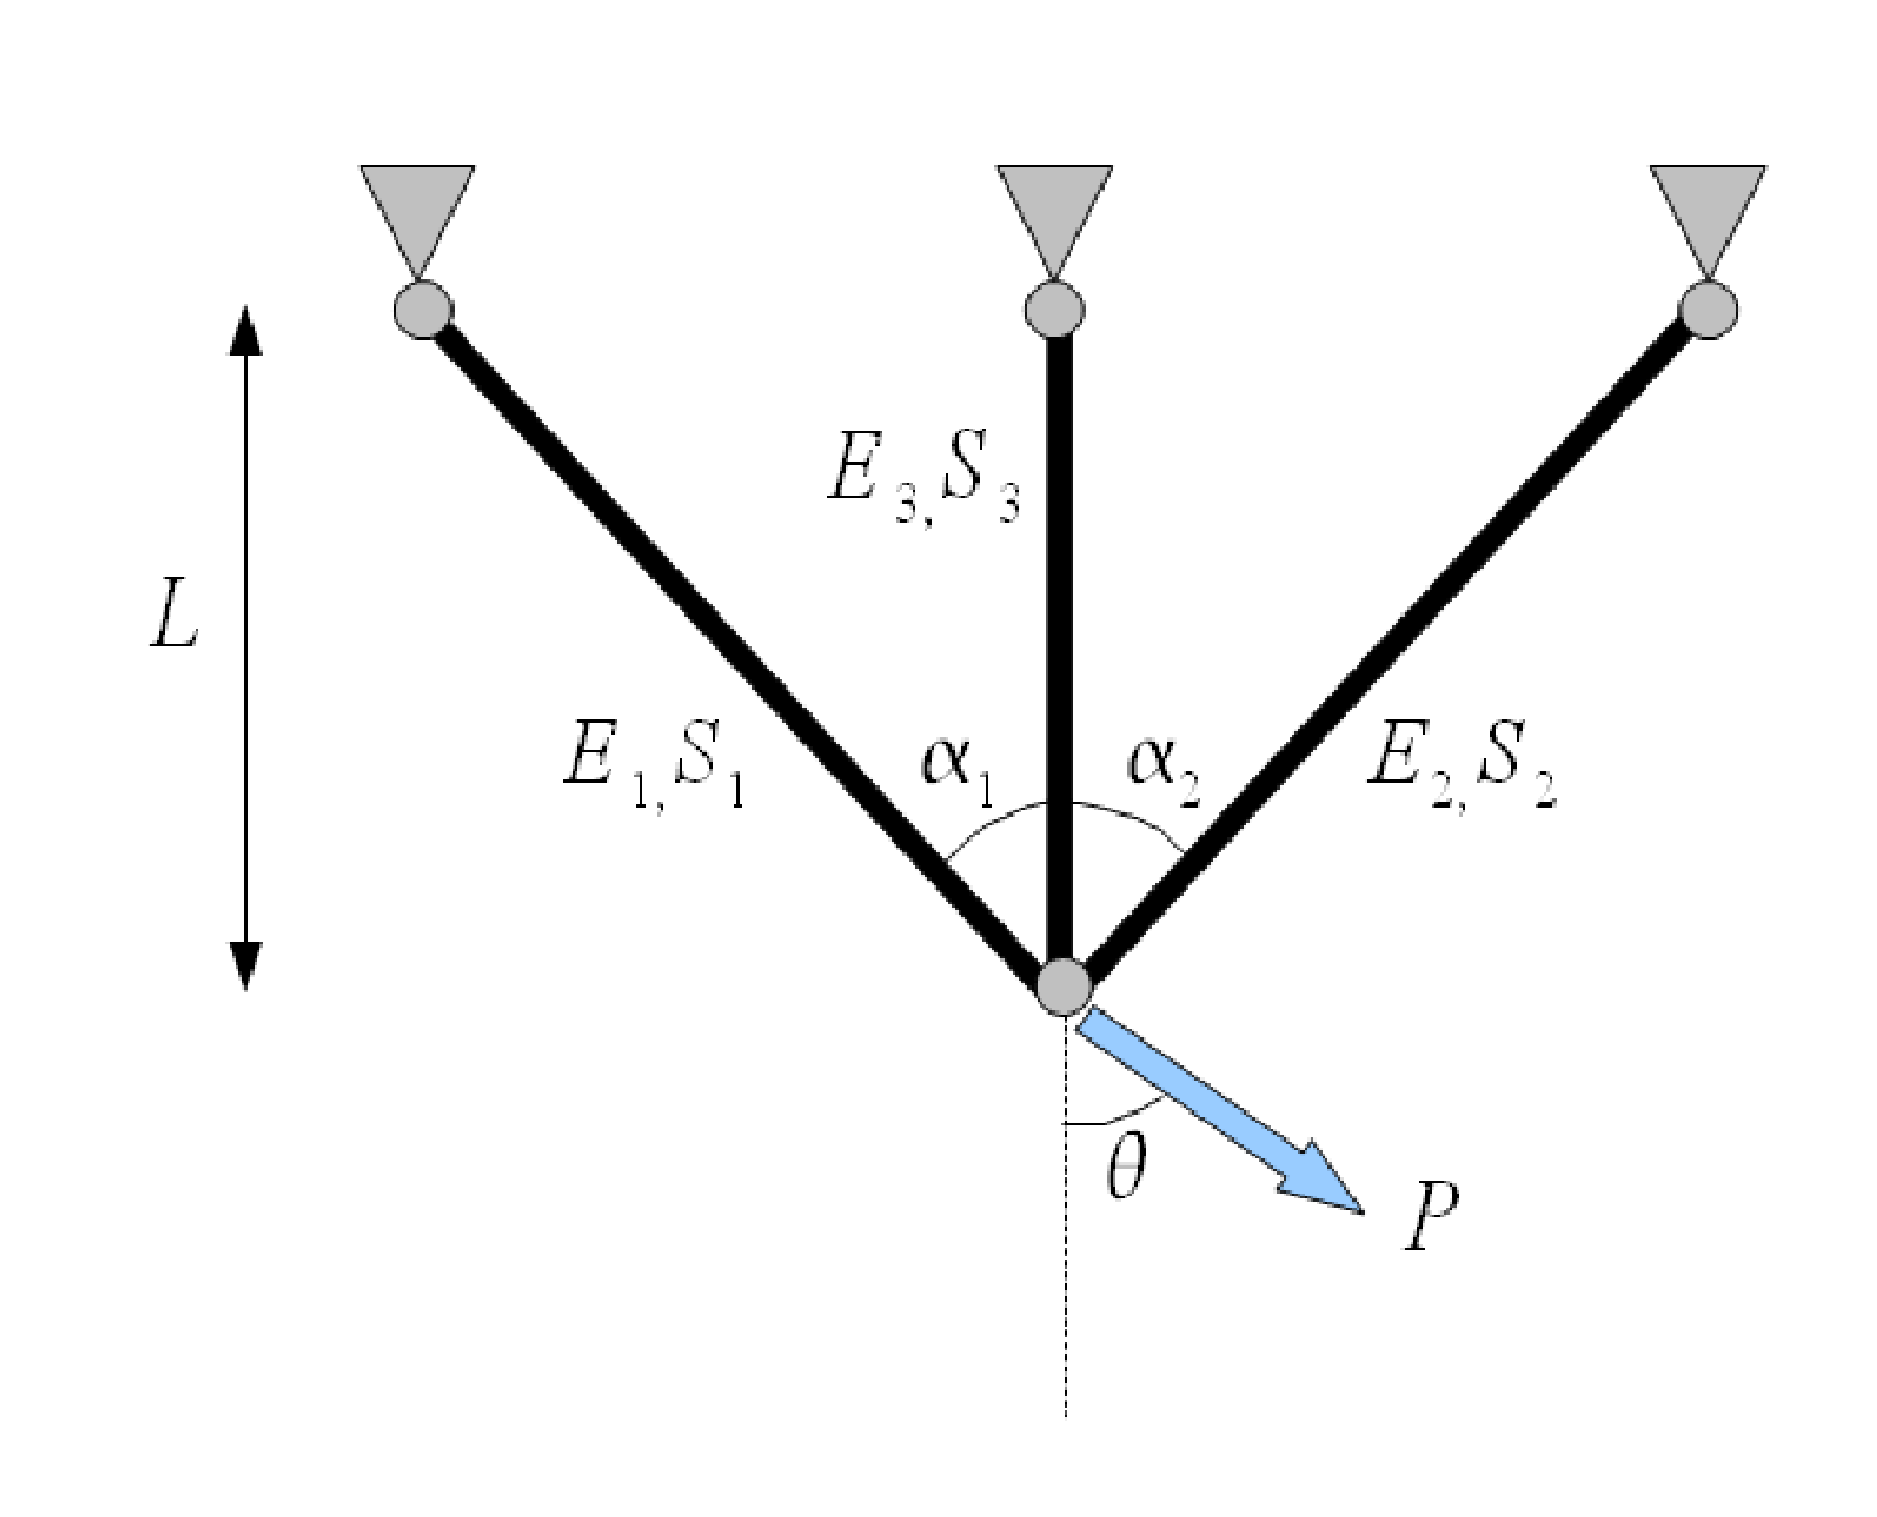
\includegraphics[width=9cm]{Figures/Treillis.pdf}
  \end{center}
  \caption{Elastic three-bar truss structure}
  \label{fig_treillis}
\end{figure}



The model response of interest is the norm $\delta$ of the displacement vector at the bottom node. It may be derived analytically as follows. The traction forces in the vertical bar (bar \#1) due to the vertical load $P_v = P \cos \theta$ and the horizontal load $P_h = P \sin \theta$ are respectively equal to:
\begin{equation}
  N_1^v \, \, = \, \, \frac{\sin(\alpha_2 + \alpha_1)}{\sin(\alpha_2)} \;
  \left[ \frac{E_3 S_3}{\cos(\alpha_1) E_1 S_1} \; + \; \frac{E_3 S_3}{\cos(\alpha_2) E_2 S_2} \left( \frac{\sin(\alpha_1)}{\sin(\alpha_2)}\right)^2 \; + \;
    \left( \frac{\sin(\alpha_1 + \alpha_2)}{\sin(\alpha_2)}\right)^2 \right]^{-1}
  \; P_v \, \, = \, \, C_v \; P_v
\end{equation}
\begin{equation}
  N_1^h \, \, = \, \,
  \frac{ \frac{\sin(\alpha_1)}{\sin(\alpha_2)^2 \cos(\alpha_2) E_2 S_2}  \; + \; \frac{\sin(\alpha_1 + \alpha_2) \cos(\alpha_2)}{\sin(\alpha_2) E_3 S_3}     }
       { \frac{1}{\cos(\alpha_1) E_1 S_1} \; + \; \frac{1}{\cos(\alpha_2) E_2 S_2} \left( \frac{\sin(\alpha_1)}{\sin(\alpha_2)}\right)^2 \; + \;
         \left( \frac{\sin(\alpha_1 + \alpha_2)}{\sin(\alpha_2)}\right)^2  \frac{1}{E_3 S_3} }
       \; P_h \, \, = \, \, C_h \; P_h
\end{equation}

Upon applying the Castigliano's theorem, the vertical and the horizontal displacements are respectively given by:
\begin{equation}
  \delta_v \, \, = \, \,
  \left[ \frac{\alpha_v^2}{E_1 S_1 \cos(\alpha_1)} \; + \; \frac{\alpha_v^2 \sin^2(\alpha_1)}{E_2 S_2 \cos(\alpha_2) \sin^2(\alpha_2)} \; + \;
    \frac{\big( 1 \; - \; \frac{\sin(\alpha_1 + \alpha_2)}{\sin(\alpha_2)}\big)^2}{E_3 S_3}  \right]
  \; P_v \; L
\end{equation}
\begin{equation}
  \delta_h  \, \, = \, \,
  \left[
    \frac{\alpha_v^2}{E_1 S_1 \cos(\alpha_1)} \; + \;  \frac{\big(\alpha_h \frac{\sin(\alpha_1)}{\sin(\alpha_2)}  \big)^2}{E_2 S_2 \cos(\alpha_2)} \; + \;
    \frac{\big(\alpha_h \frac{\sin(\alpha_1 + \alpha_2)}{\sin(\alpha_2)} \; - \; \frac{\cos(\alpha_2)}{\sin(\alpha_2)} \big)^2}{E_3 S_3}
    \right]
  \; P_h \; L
\end{equation}
where $L$ denotes the length of bar \#3. Eventually the model response of interest $\delta$ is the Euclidean norm of the displacement, that is:
\begin{equation}
  \delta \, \, = \, \, \sqrt{\delta_h^2 \; + \; \delta_v^2}
\end{equation}

\subsubsection{Probabilistic model}

The cross-section areas, the Young's moduli, the point load and the angles are assumed to be uncertain and are modelled by independent random variables. Hence an input random vector of dimension $M=10$ and which reads:
\begin{equation}
  \underline{X} \, \, = \, \, \{E_1,E_2,E_3,S_1,S_2,S_3,P,\alpha_1,\alpha_2,\theta\}^{\mbox{\textsf{T}}}
\end{equation}
The distributions and the parameters of the random variables are reported in Table~\ref{table_rvs}.


\begin{table}[Hhbtp]
  \begin{center}
    \begin{tabular}{cccc}
      \hline
      Variable & Distribution & Mean & Coef. of variation \\
      \hline
      $E_i$ &  Lognormal & $210 \;$ GPa& $10\%$ \\
      $S_i$ & Normal & $1.5\cdot 10^{-3}\;$ m$^2$ & $5\%$ \\
      $P$ & Gumbel & $2.5\cdot10^{5}\;$ N& $20\%$ \\
      $\alpha_j$ & Normal & $45^\circ$& $3\%$\\
      $\theta$ & Normal & $45^\circ$& $3\%$   \\
      \hline
    \end{tabular}
    \caption{Three-bar truss example -- Input random variables}
    \label{table_rvs}
  \end{center}

\end{table}

Due to uncertainty propagation through the model $\cM$, the displacement (i.e. the model response) is also a random variable denoted by $Y = \cM(\underline{X})$. The characterization of the distribution of $Y$ and of some of its properties (e.g. moments, sensitivity indices) are of interest in the sequel.

\subsection{Uncertainty and sensitivity analysis based on polynomial chaos expansions}

\subsubsection{Methodology to construct a sparse polynomial chaos approximation}

\paragraph{}
In order to perform uncertainty and sensitivity analysis at a low computational cost, we aim at constructing a polynomial chaos (PC) approximation of the model response. In this purpose, the input parameters $X_i$ are first scaled according to the following isoprobabilistic transform:
\begin{equation}
  \xi_i \, \, = \, \, \Phi^{-1}(F_{X_i}(X_i)) \, \quad \; , \quad i=1,\dots,10
\end{equation}
where $\Phi$ and $F_{X_i}$ denote the cumulative density function of the standard normal distribution and the variable $X_i$, respectively. This makes it possible to recast the random model response (denoted by $Y$) in terms of independent standard normal random variables $\underline{\xi} = \{\xi_1,\dots,\xi_{10}\}$ as follows:
\begin{equation}
  Y \, \, = \, \, \cM(\underline{\xi})
\end{equation}

\paragraph{}
We want to approximate the model response $Y$ by a PC expansion made of normalized Hermite polynomials. Such a representation reads:
\begin{equation}
  Y \, \, \simeq \, \, Y^\textsf{PC} \, \, = \, \, \sum_{\underline{\alpha} \in \Lambda} \; a_{\underline{\alpha}} \; \psi_{\underline{\alpha}}(\underline{\xi})
\end{equation}
In the above equation, $\psi_{\underline{\alpha}}(\underline{\xi})$ is a product of normalized Hermite polynomials, that is:
\begin{equation}
  \psi_{\underline{\alpha}}(\underline{\xi}) \, \, = \, \, \prod_{i=1}^M \; H_{\alpha_i}(\xi_i)
\end{equation}
where $H_{\alpha_i}$ is the normalized Hermite polynomial of degree $\alpha_i$. $\Lambda$ is a non empty and finite subset of $\Nset^M$. The $a_{\underline{\alpha}}$'s are the PC coefficients that have to be estimated.

\paragraph{}
It is assumed that the maximum number of allowed simulations (i.e. the simulation budget) is equal to $N=200$. We want to make the best use of these model evaluations to construct a PC approximation of the response. To this end, several PC expansions are built up for various total degrees $p$ ranging from 1 to 4 (thus the so-called \emph{fixed strategy} is used to truncate all of these metamodels). It is recalled that the number of terms in these approximations is given by the formula:
\begin{equation}
  P \quad = \quad \frac{(M+p)!}{M!p!}
\end{equation}
It has to be noted that $P>N$ when the degree $p$ is greater than or equal to 3 ($P$ is equal to $286$ if $p=3$ and to $1,001$ if $p=4$). As a consequence, it is not possible to evaluate the PC coefficients by \emph{ordinary least squares} in this case since the problem would be ill-posed. As an alternative, the coefficients are computed using a \emph{sparse least squares} approach based on \emph{least angle regression} (LAR). In this purpose, the $N$ simulations are carried out in such a way that the corresponding $N$ realizations of the input random vector $\underline{X}$ form a \emph{latin hypercube design}.

\subsubsection{Parametric study varying the degree of the metamodel}

\paragraph{}
The LAR approach is used to compute the coefficients of the PC approximations of degrees $p$ varying from 1 to 4. Then these metamodels are assessed by evaluating their \emph{corrected leave-one-out errors} (these quantity are calculated when running LAR and are hence available as a by-product of this algorithm). The errors are plotted in Figure~\ref{fig_errors}.

\begin{figure}[Hhbtp]
  \begin{center}
    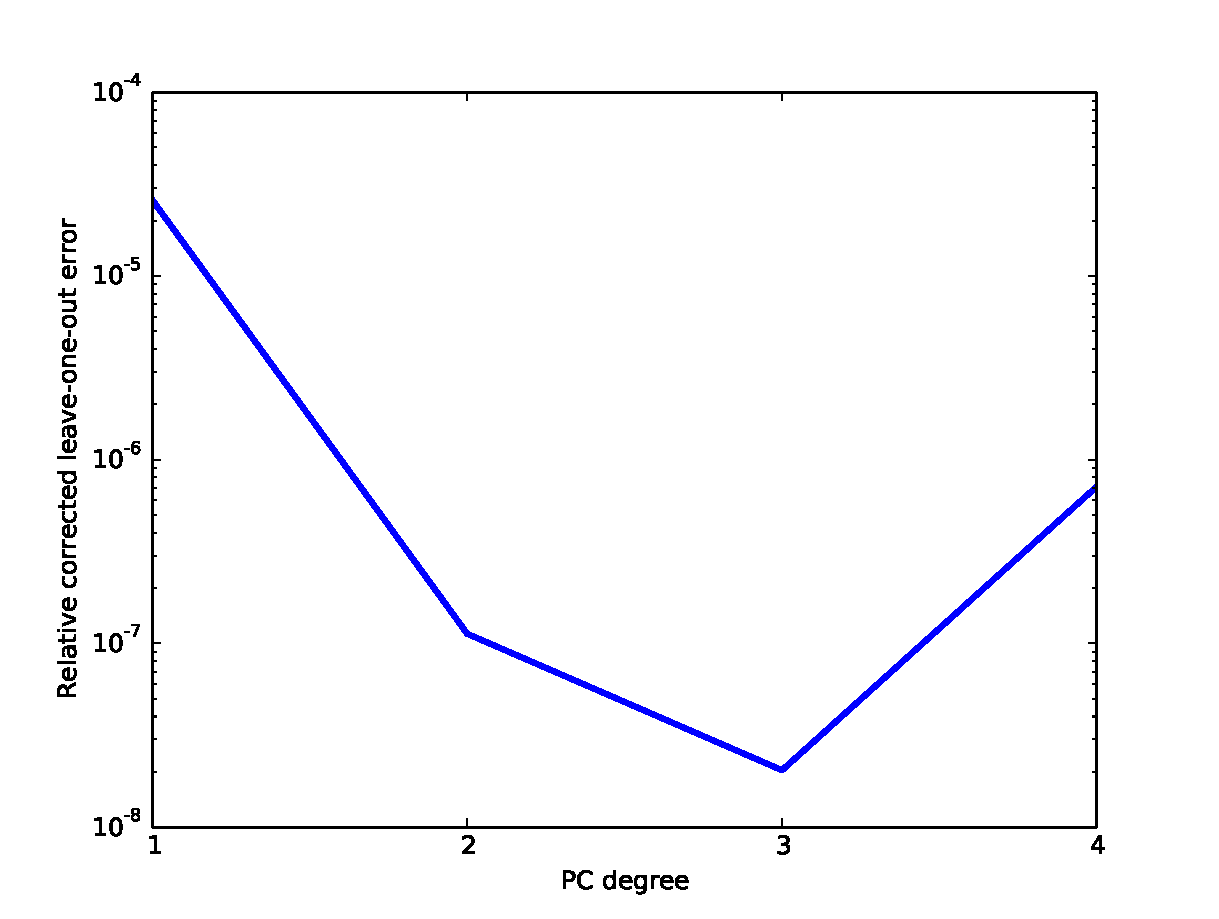
\includegraphics[width=12cm]{Figures/Truss_errors.pdf}
  \end{center}
  \caption{Corrected leave-one-out errors associated with the various polynomial chaos approximations}
  \label{fig_errors}
\end{figure}

It appears that the PC of degree $p=3$ is the most accurate, with an error estimate equal to $1.2 \cdot 10^{-4}$. It contains $P'=97$ non zero coefficients, that is a ``sparsity ratio'' equal to $97 / 286~\approx~ 34\%$ compared to the total number of coefficients.

\subsubsection{Second moments and sensitivity indices based on chaos coefficients}

From now on, we only consider the sparse PC expansion of degree $p=3$. It is straight forward to estimate the mean and the standard deviation of the random displacement $Y$ from the PC coefficients:
\begin{equation}
  \mu_{Y^\textsf{PC}} \quad \approx \quad 4.3~\mbox{mm} \qquad , \qquad \sigma_{Y^\textsf{PC}} \quad \approx \quad 0.9~\mbox{mm}
\end{equation}
hence a coefficient of variation equal to $21\%$. \\

The sensitivity indices of $Y$ to each input random variable $X_i$ can also be computed easily from the coefficients. The \emph{single-effect} indices are plotted together with the \emph{total} ones in Figure~\ref{fig_SA}.

\begin{figure}[Hhbtp]
  \begin{center}
    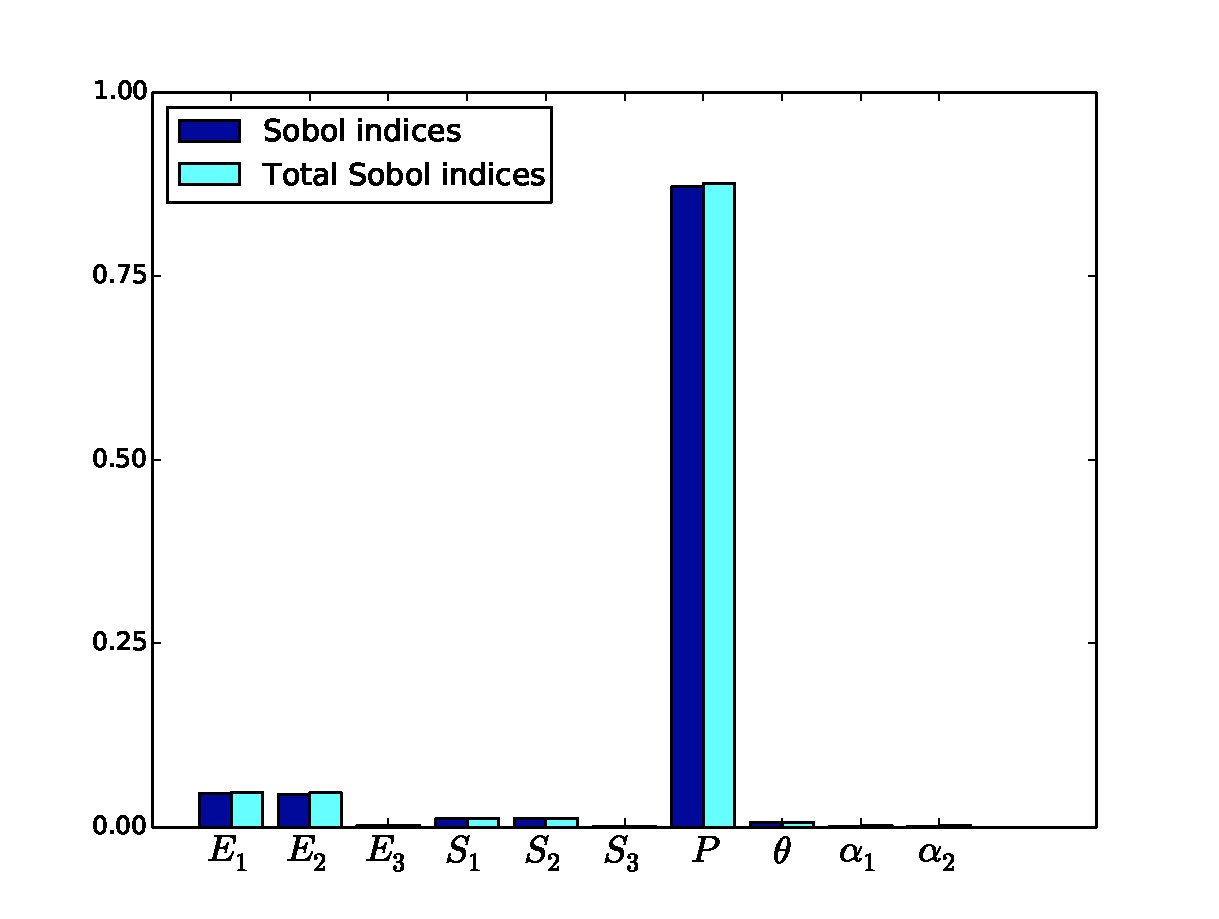
\includegraphics[width=12cm]{Figures/Truss_SA.pdf}
  \end{center}
  \caption{Single-effect and total sensitivity indices of the truss displacement to the various input parameters}
  \label{fig_SA}
\end{figure}

It is observed that both kinds of indices strongly coincidate, which reveals that there is almost no interaction effect. The variability of $Y$ is mainly explained by the one of the point load $P$. Indeed, the associated sensitivity indices are both nearly equal to $90\%$. On the contrary, all the input variables except the Young's moduli $E_1$ and $E_2$ have a negligible influence on the variance of $Y$, with sensitivity indices less than $2\%$. Therefore, it would be relevant in further investigation to fix all the insignificant variables to their nominal values, and to focus on a fine characterization of the distribution of the load $P$.

\subsubsection{Distribution and higher-order moments analysis}

Of interest is the estimation of the probability density function (PDF) of $Y$ by exploiting its PC approximation $Y^\textsf{PC}$, which is very fast to evaluate. Note that in this example the original model is itself fast to simulate, for it is formulated in terms of a closed-form equation Hence the computational gain related to the use of a metamodel is not really significant. Nonetheless, such a gain would be considerable in presence of a more complicated model, e.g. a finite element model with many degrees of freedom. This is why we nevertheless decided to use the metamodel-based methodology in the following. \\

First, a large sample of size $\cN = 100,000$ is drawn according to the joint distribution of the input random vector $\underline{X}$. Then the PC metamodel is evaluated at each input realization, leading to a $\cN$-sample of responses. The histogram of this sample is represented in Figure~\ref{fig_histo}. From visual inspection, the PDF of $Y$ appears to be slightly positively skewed. \\

\begin{figure}[Hhbtp]
  \begin{center}
    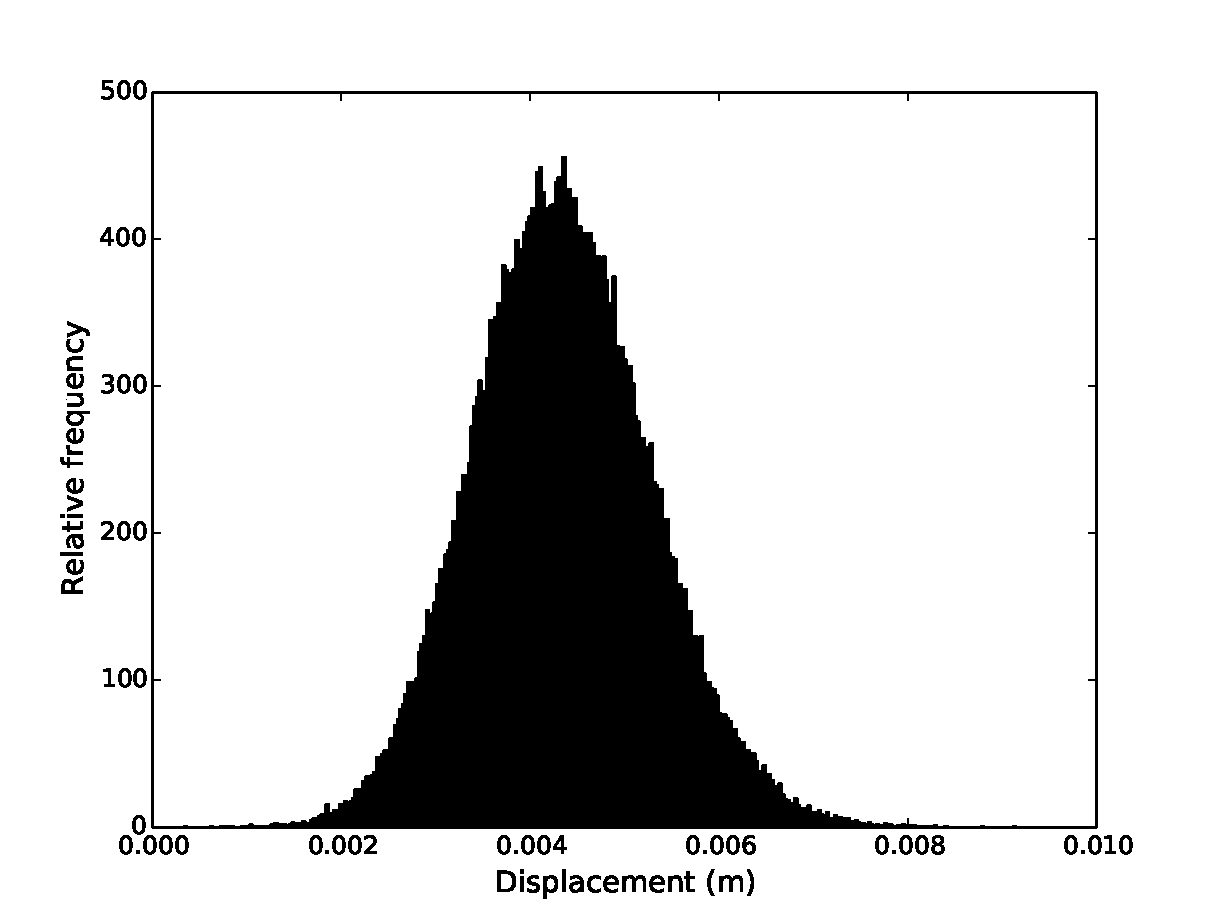
\includegraphics[width=12cm]{Figures/Truss_histo.pdf}
  \end{center}
  \caption{Histogram of the random displacement}
  \label{fig_histo}
\end{figure}

The sample standardized moments of order 3 and 4, namely the \emph{skewness} and \emph{kurtosis} coefficients, are given by:
\begin{equation}
  \gamma_{1,Y^\textsf{PC}} \quad \approx \quad 0.15 \qquad , \qquad \gamma_{2,Y^\textsf{PC}} \quad \approx \quad 3.09
\end{equation}
Broadly speaking, the random variable $Y$ is not so far from a Gaussian distribution, for which the skewness and the kurtosis would be equal to 0 and 3, respectively. This could be expected since even a PC of degree $p=1$ had an approximation error of only $7 \cdot 10^{-3}$ (Figure~\ref{fig_errors}). In other words, a linear combination of Gaussian variables $\xi_i$, which is itself a Gaussian variable, revealed a fair approximation of the model response.

\subsection{Python scripts}

The Python files include two modules corresponding to the physical and the probabilistic models, and one main program which performs the uncertainty analysis based on polynomial chaos expansions.

\subsubsection{Physical model -- \textsf{scriptExample\_Truss\_PhysicalModel.py}}
\lstinputlisting{scriptExample_Truss_PhysicalModel.py}

\subsubsection{Probabilistic model -- \textsf{scriptExample\_Truss\_ProbaModel.py}}
\lstinputlisting{scriptExample_Truss_ProbaModel.py}

\subsubsection{Uncertainty analysis based on PC expansions -- \textsf{scriptExample\_Truss\_mainSparsePolyChaos.py}}
\lstinputlisting{scriptExample_Truss_mainSparsePolyChaos.py}


\end{document}
